\subsection{模的投射覆盖}

定义 3. —— 设 A 是一个环，M 是一个 A-模。M 的投射覆盖是指一个偶 \((P, u)\)，其中 P 是一个投射 A-模，u 是从 P 到 M 的一个满同态，使得 \(u(P') \neq M\) 对 P 的每个真 A-子模 \(P'\) 成立。

注. —— 1) 对每个投射 A-模 M，偶 \((M,1_{M})\) 是 M 的一个投射覆盖。

\begin{enumerate}
\def\labelenumi{\arabic{enumi})}
\setcounter{enumi}{1}
\tightlist
\item
  设 \((\mathrm{P}, u)\) 是 A-模 M 的一个投射覆盖。设 \((x_{i})_{i \in \mathrm{I}}\) 是 P 的元素的一个族，\(P'\) 是它生成的 P 的子模；则 \(u(\mathrm{P}')\) 由族 \((u(x_{i}))_{i \in \mathrm{I}}\) 生成。因而，族 \((x_{i})_{i \in \mathrm{I}}\) 生成 A-模 P 当且仅当族 \((u(x_{i}))_{i \in \mathrm{I}}\) 生成 A-模 M。特别地，P 是有限生成的当且仅当 M 是有限生成的。
\end{enumerate}

命题 8. —— 设 M 与 M' 是 A-模，(P, u) 与 (P', u') 分别是 M 与 M' 的投射覆盖，g : M → M' 是一个 A-线性映射。

\begin{enumerate}
\def\labelenumi{\alph{enumi})}
\item
  存在一个 A-线性映射 \(f: \mathrm{P} \to \mathrm{P}'\)，使得 \(u' \circ f = g \circ u\)。
\item
  设 f 是这样一个映射。若 g 是满射（相应地，双射），则 f 是满射（相应地，双射）。若 g 是单射且其像是 \(M'\) 的一个直因子，则 f 是单射且其像是 \(P'\) 的一个直因子。
\end{enumerate}

根据假设，A-模 P 是投射的，且映射 \(u'\) 是满射。于是，存在一个 A-线性映射 \(f: P \to P'\)，使得 \(g \circ u = u' \circ f\)（II, §2, No.~2, 第 231 页，命题 4）。断言 a) 由此得出。

设 \(f\) 是 a) 中那样的一个映射。假设 \(g\) 是满射。由于 \(u\) 是满射，我们有 \(M' = g(u(P)) = u'(f(P))\)。由于 \((P', u')\) 是 \(M'\) 的一个投射覆盖，我们有 \(f(P) = P'\)，故 \(f\) 是满射。由同前所引，\(f\) 的核有一个补子模 \(P_1\)，于是 \(f(P_1) = P'\)。现在假设 \(g\) 是双射。我们有 \(g(u(P_1)) = u'(f(P_1)) = u'(P') = M'\)，从而 \(u(P_1) = M\)。由于 \((P, u)\) 是 \(M\) 的一个投射覆盖，我们有 \(P_1 = P\)，因而 \(\text{Ker}(f) = 0\)。所以 \(f\) 是单射；由于已知 \(f\) 是满射，故 \(f\) 是双射。

最后，假设 \(g\) 是单射且其像是 \(\mathrm{M}'\) 的一个直因子。那么存在一个 A-线性映射 \(g': \mathrm{M}' \to \mathrm{M}\)，使得 \(g' \circ g = 1_{\mathrm{M}}\)。由 a)，存在一个 A-线性映射 \(f': \mathrm{P}' \to \mathrm{P}\)，使得 \(u \circ f' = g' \circ u'\)。我们有 \(u \circ (f' \circ f) = g' \circ u' \circ f = (g' \circ g) \circ u\)；由上一段知，映射 \(f' \circ f\) 是双射。用 h 表示其逆双射；我们有 \((h \circ f') \circ f = 1_{\mathrm{P}}\)，故 f 是单射，且其像是 \(P'\) 的一个直因子（II, §1, No.~9, 第 212 页，推论 2）。

推论 1. —— 设 M 是一个 A-模。设 \((P, u)\) 与 \((P', u')\) 是 M 的投射覆盖。存在一个从 P 到 \(P'\) 的同构 f，使得 \(u = u' \circ f\)。

\pandocbounded{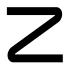
\includegraphics[keepaspectratio]{images/part001_525bb1e1.jpg}}

注意，f 不一定由关系式 \(u = u' \circ f\) 唯一确定（VIII, 第 170 页，习题 21）。

推论 2. —— 设 \((\mathrm{P}, u)\) 是 A-模 M 的一个投射覆盖。若 Q 是一个投射 A-模，且 \(g : Q \to M\) 是一个满线性映射，则存在一个满线性映射 \(f : Q \to P\)，使得 \(g = u \circ f\)。

命题 9. —— 设 M 是一个 A-模，\((P, u)\) 是 M 的一个投射覆盖。用 r 表示环 A 的根。由 u 取商得到的同态 \(\overline{u}: P/rP \to M/rM\) 是一个同构。

同态 \(u\) 按定义是满射，故 \(\overline{u}\) 是满射。将 \(u\) 的核记作 \(N\)。我们有 \(u^{-1}(\mathfrak{rM}) = N + \mathfrak{rP}\)。我们来证明 \(N \subset \mathfrak{rP}\)，由此即得 \(\overline{u}\) 的单射性。设 \(P'\) 是 \(P\) 的一个极大子模；我们有 \(u(P') \neq M\)，因而 \(P' + N \neq P\)；由于 \(P'\) 是极大的，我们有 \(N \subset P'\)。于是 \(N\) 作为 \(P\) 的子模含于 \(P\) 的根中。而后者由 VIII, 第 158 页的命题 6 等于 \(\mathfrak{rP}\)。

推论. —— 若 A-模 M 具有一个投射覆盖，则 A/r-模 M/rM 是投射的。

事实上，若 \((P,u)\) 是 M 的一个投射覆盖，则 \((A/\mathfrak{r})\)-模 M/rM 同构于 P/rP（命题 9）。由于 A-模 P 是投射的，\((A/\mathfrak{r})\)-模 P/rP 也是投射的。

注. —— 3) 假设环 A 无根。由命题 9，\((P, u)\) 是 A-模 M 的一个投射覆盖当且仅当 u 是同构。因此，只有投射 A-模才可能具有投射覆盖。

环 Z 无根（VIII, 第 154 页，例 3）。设 \(n \geqslant 2\) 是一个整数。Z-模 Z/nZ 不是投射的，因而不具有投射覆盖。

\begin{enumerate}
\def\labelenumi{\arabic{enumi})}
\setcounter{enumi}{3}
\tightlist
\item
  假设每个有限生成 A-模都具有一个投射覆盖；则 A 对其根的商 \(A'\) 是半单的。事实上，由该推论，环 \(A'\) 上的每个有限生成模都是投射的。特别地，若 \(\mathfrak{a}\) 是 \(A'\) 的一个左理想，则 \(A'\)-模 \(A_s'/\mathfrak{a}\) 是投射的。于是我们的断言由 VIII, 第 138 页的命题 4 得出。
\end{enumerate}

我们可以给出这样的例子：一个交换环 A，使得 A/r 是半单的，以及一个不具有投射覆盖的有限生成 A-模 M（VIII, 第 170 页，习题 22）。

命题 10. —— 设 M 是一个 A-模，P 是一个投射 A-模，\(u : P \to M\) 是一个线性映射。设 a 是 A 的一个双边理想。假设由 u 取商得到的线性映射 \(\overline{u} : P / aP \to M / aM\) 是双射，且下列条件之一成立：

\begin{enumerate}
\def\labelenumi{(\roman{enumi})}
\item
  A-模 M 与 P 都是有限生成的，且 a 含于 A 的根中。
\item
  理想 \(\mathfrak{a}\) 是幂零的。
\end{enumerate}

则 (P, u) 是 M 的一个投射覆盖。

在这些假设下，同态 \(u\) 是满射（VIII, 第 159 页，推论 2），且其核 \(N\) 含于 \(\mathfrak{a}P\)。设 \(P'\) 是 \(P\) 的一个真子模。由中山引理（VIII, 第 158 页，定理 2），我们有 \(P' + \mathfrak{a}P \neq P\)，因而 \(u(P') \neq M\)。所以 \((P, u)\) 是 \(M\) 的一个投射覆盖。

推论 1. —— 设 P 是一个投射 A-模。假设 P 是有限生成的，或者 A 的根 r 是一个幂零双边理想。用 u 表示从 P 到 P/rP 的典范映射。则 (P, u) 是 P/rP 的一个投射覆盖。

推论 2. —— 设 a 是 A 的一个双边理想，M 是一个 A-模，使得 (A/a)-模 M/AM 是自由的。假设下列条件之一成立：

\begin{enumerate}
\def\labelenumi{(\roman{enumi})}
\item
  模 M 是有限生成的，且 \(\mathfrak{a}\) 含于 A 的根中。
\item
  理想 \(\mathfrak{a}\) 是幂零的。
\end{enumerate}

则 M 具有一个投射覆盖。

更精确地说，设 P 是一个自由 A-模，\((e_{i})_{i\in\mathrm{I}}\) 是 P 的一个基，\(u:P\to M\) 是一个同态，使得 M/aM 的元素 \(u(e_{i})\) 的典范像构成 (A/a)-模 M/aM 的一个基。则 (P,u) 是 M 的一个投射覆盖。

\((\mathrm{A}/\mathfrak{a})\)-模 P/aP 是自由的，而由 u 取商得到的从 P/aP 到 M/aM 的同态 \(\overline{u}\) 把 P/aP 的一个基变成 M/aM 的一个基，因而是双射。

若 a 是幂零的，则只需应用命题 10。现在假设环 A 非零且模 M 是有限生成的；则 \((A/a)\)-模 M/aM 也是有限生成的，从而 \((A/a)\)-模 P/aP 亦然。于是 P/aP 的每个基都是有限的。由此推出集 I 是有限的，且 A-模 P 是有限生成的。然后再一次应用命题 10。

推论 3. —— 局部环上的每个有限生成模都具有一个投射覆盖。

设 A 是一个局部环，r 是它的根。它是 A 的一个双边理想（VIII, 第 155 页，命题 5, a)），且环 A/r 是一个体（VIII, 第 157 页，推论 4）。若 M 是一个 A-模，则 M/rM 是体 A/r 上的一个向量空间，因而是一个自由 (A/r)-模。于是只需应用推论 2。

注 5. —— 设 A 是一个局部环，r 是它的根。设 M 是一个有限生成 A-模，P 是一个有限生成投射 A-模，\(u : P \to M\) 是一个同态。由 VIII, 第 36 页的推论 6，A-模 P 是自由的。选取 P 的一个基 \((e_{i})_{i \in I}\)。令 \(x_{i} = u(e_{i})\)，且将 \(x_{i}\) 在 M/rM 中的典范像记作 \(\overline{x}_{i}\)。下列性质等价：

\begin{enumerate}
\def\labelenumi{(\roman{enumi})}
\item
  偶 \((\mathrm{P},u)\) 是 M 的一个投射覆盖。
\item
  族 \((x_{i})_{i\in \mathrm{I}}\) 是 A-模 M 的一个极小生成族。
\item
  族 \((\overline{x}_{i})_{i\in\mathrm{I}}\) 是体 A/r 上的向量空间 M/rM 的一个基。
\end{enumerate}

由 VIII, 第 161 页的注 2 得 (i) \(\Rightarrow\) (ii)，由推论 2 得 (iii) \(\Rightarrow\) (i)。此外，若族 \((x_{i})\) 是 A-模 M 的一个极小生成族，则族 \((\overline{x}_{i})\) 是 A/r 上的向量空间 M/rM 的一个极小生成族，即一个基（VIII, 第 158 页，推论 1）。

命题 11. —— 设 A 是一个环，a 是 A 的一个幂零双边理想。设 M 是一个投射 A/a-模。存在一个投射 A-模 P 和一个核为 aP 的满 A-线性映射 \(u: \mathrm{P} \to \mathrm{M}\)。

把 M 视为 A-模时，这样的一个偶 \((P,u)\) 是 M 的一个投射覆盖。

存在一个 A/ \(\alpha\)-模 \(M'\)，使得 \(M \oplus M'\) 是一个自由 A/ \(\alpha\)-模。选取一个自由 A-模 L 和一个核为 aL 的满 A-线性映射 \(v: L \to M \oplus M'\)。由命题 7 的推论 1（VIII, 第 159 页），存在一个直和分解 \(L = P \oplus P'\)，使得 \(v(P) = M\) 且 \(v(P') = M'\)。A-模 P 是投射的，而在 P 上与 v 一致的从 P 到 M 的 A-线性映射 u 是满射，其核为 aP。第一个断言由此得出。

设 P 是一个投射 A-模，u 是一个从 P 到 M 的核为 aP 的同态。由命题 10，偶 \((P,u)\) 是 M 的一个投射覆盖。

推论. —— 设 P 与 P' 是投射 A-模。若模 P/ \(\alpha\) P 与 P'/ \(\alpha\) P' 同构，则 P 与 P' 同构。

由于 P/aP 与 \(P^{\prime}/aP^{\prime}\) 都是投射的，该推论由命题 11 及投射覆盖的唯一性（VIII, 第 162 页，推论 1）得出。

\BourbakiExercises{习题}

\begin{enumerate}
\def\labelenumi{\arabic{enumi})}
\tightlist
\item
  设 \(\mathrm{K}\) 是一个特征为 \(p\) 的交换域，\(\mathrm{M}\) 是一个 \(p\)-准素 \(\mathbf{Z}\)-模，\(\mathrm{A}\) 是群 \(\mathrm{M}\) 在 \(\mathrm{K}\) 上的代数，\(\mathfrak{m}\) 是元素 \(\sum_{m} a_{m} e_{m}\)（属于 \(\mathrm{A}\)，参见 III, §2, No.~6, 第 446 页）中满足 \(\sum_{m} a_{m} = 0\) 者所成的集。
\end{enumerate}

\begin{enumerate}
\def\labelenumi{\alph{enumi})}
\item
  证明 A 是一个局部环，其极大理想为 \(\mathfrak{m}\)，并且 \(\mathfrak{m}\) 是一个诣零理想（参见 VIII, 第 41 页，习题 10）。
\item
  此外，假设位似 \(p_{\mathrm{M}}\) 是满射。证明我们有 \(\mathfrak{m} = \mathfrak{m}^2\)。
\end{enumerate}

\begin{enumerate}
\def\labelenumi{\arabic{enumi})}
\setcounter{enumi}{1}
\item
  设 A 是一个环，M 是一个无根 A-模。证明位似环 \(A_{M}\) 无根（把 \(A_{s}\) 与 \(M^{M}\) 的一个子模等同起来）。
\item
  \begin{enumerate}
  \def\labelenumii{\alph{enumii})}
  \tightlist
  \item
    设 A 是一个环，其商环 \(\mathrm{A} / \Re (\mathrm{A})\) 是半单的。证明对每个 A-模 M，我们有 \(\Re (\mathrm{M}) = \Re (\mathrm{A})\mathrm{M}\)（注意 \(\mathrm{M} / \Re (\mathrm{A})\mathrm{M}\) 是一个 \(\mathrm{A} / \Re (\mathrm{A})\)-模）。
  \end{enumerate}
\end{enumerate}

\begin{enumerate}
\def\labelenumi{\alph{enumi})}
\setcounter{enumi}{1}
\tightlist
\item
  由此给出一个环 A 和一个 A-模的族 \((\mathrm{V}_{i})_{i\in\mathrm{I}}\) 的例子，使得 \(\Re\big(\prod\mathrm{M}_{i}\big)\neq\prod\Re(\mathrm{M}_{i})\)（对一个根不是有限生成的环利用 a)）。
\end{enumerate}

\begin{enumerate}
\def\labelenumi{\arabic{enumi})}
\setcounter{enumi}{3}
\item
  设 A 是一个交换域 K 上的代数，a 是 A 的一个双边理想。设 B 是由 1 与 a 生成的 A 的子代数。证明 B 的根含于 A 的根之中（注意若 S 是一个单 A-模，则或者对每个 \(x \in S\) 有 ax = 0，或者对 S 中每个 \(x \neq 0\) 有 ax = S）。
\item
  设 \(A\) 是一个交换域 \(K\) 上的代数。
\end{enumerate}

\begin{enumerate}
\def\labelenumi{\alph{enumi})}
\tightlist
\item
  证明 A 的根中在 K 上为代数元的元素是幂零的。b) 假设 K 是一个无限域且 \(\operatorname{Card}(K) > [A : K]\)。证明 A 的根是一个诣零理想（按 VIII, 第 47 页的引理 1 的方式论证）。
\end{enumerate}

\begin{enumerate}
\def\labelenumi{\arabic{enumi})}
\setcounter{enumi}{5}
\tightlist
\item
  设 \(\mathrm{A}\) 是一个环。
\end{enumerate}

\begin{enumerate}
\def\labelenumi{\alph{enumi})}
\item
  设 \(\mathfrak{a}\) 与 \(\mathfrak{b}\) 是 A 的双边理想。若 \(\mathfrak{a}\) 与 \(\mathfrak{b}\) 都是幂零的（相应地，诣零理想），则 \(\mathfrak{a} + \mathfrak{b}\) 亦然。
\item
  证明所有双边诣零理想之和 \(\mathfrak{G}\) 是一个双边诣零理想，而所有幂零双边理想之和 \(\mathfrak{N}\) 是一个包含所有幂零理想的双边诣零理想（VIII, 第 149 页，习题 3）。
\item
  证明 G 是 A 的最大半素诣零理想（同前所引）；我们称 G 为 A 的幂零根。若 A 是交换的，则 G 与 N 都等于 A 的幂零元素所成之集。
\end{enumerate}

¶ 7) 设 A 是一个环，I 是这样的序数 \(\alpha\) 所成之集：\(\text{Card}(\alpha) \leqslant \text{Card}(A)\)（《集合论》，III, §6, 第 241 页，习题 10）。用超限归纳定义双边理想 \(\mathfrak{N}_{\alpha}\)（对每个 \(\alpha \in I\)）如下。取 \(\mathfrak{N}_0 = \mathfrak{N}\)（习题 6, b)）。若 \(\alpha\) 有后继 \(\alpha + 1\)，则 \(\mathfrak{N}_{\alpha+1}\) 是使 \(\mathfrak{N}_{\alpha+1}/\mathfrak{N}_{\alpha}\) 为 \(A/\mathfrak{N}_{\alpha}\) 的诸幂零双边理想之和的双边理想。若 \(\alpha\) 是一个极限序数，则取 \(\mathfrak{N}_{\alpha}\) 为诸 \(N_{\beta}\)（\(\beta < \alpha\)）的并。设 \(\tau\) 是使 \(N_{\tau+1} = N_{\tau}\) 的最小序数；理想 \(P = N_{\tau}\) 称为 A 的素根。

\begin{enumerate}
\def\labelenumi{\alph{enumi})}
\item
  证明我们有 \(N \subset P \subset G\)，且 P 是 A 的最小半素诣零理想。\(^{(1)}\)
\item
  证明 \(\mathfrak{P}\) 是 A 的诸半素双边理想的交（参见 VIII, 第 149 页，习题 3）。
\item
  证明 P 是 A 的诸素双边理想的交（同前所引，c)）。d) 证明 P 是 A 中具有下述性质的元素 a 所成之集：A 中元素的每个序列 \((a_{n})_{n\geqslant0}\)，若它满足 \(a_{0}=a\) 且对每个 n 有 \(a_{n+1}\in a_{n}Aa_{n}\)，则它具有有限支集（方法同同前所引）。
\end{enumerate}

\begin{enumerate}
\def\labelenumi{\arabic{enumi})}
\setcounter{enumi}{7}
\tightlist
\item
  我们沿用习题 7 的记号。设 A 是一个左诺特环。
\end{enumerate}

\begin{enumerate}
\def\labelenumi{\alph{enumi})}
\item
  证明 \(\mathfrak{N}\) 是 A 的最大幂零双边理想，且它等于 A 的素根 \(\mathfrak{P}\)。
\item
  证明 A 的每个左或右诣零理想都是幂零的（对环 A/N 应用 VIII, 第 150 页的习题 5, a)）。于是我们有 \(\mathfrak{N} = \mathfrak{P} = \mathfrak{G}\)。
\end{enumerate}

\begin{enumerate}
\def\labelenumi{\arabic{enumi})}
\setcounter{enumi}{8}
\item
  设 \(\mathrm{K}\) 是一个交换域，\(\mathrm{B}\) 是环 \(\mathrm{K}[(\mathrm{X}_n)_{n\geqslant 1}]\)，\(\mathfrak{I}\) 是 \(\mathrm{B}\) 中由序列 \((\mathrm{X}_n^n)\) 生成的理想，\(\mathrm{A}\) 是环 \(\mathrm{B} / \mathfrak{I}\)。证明 \(\mathrm{A}\) 的根是一个诣零理想但不是幂零的。
\item
  设 A 是一个环。
\end{enumerate}

\begin{enumerate}
\def\labelenumi{\alph{enumi})}
\item
  设 Z 是 A 的中心。证明我们有 \(Z \cap \Re(A) \subset \Re(Z)\)（参见下文习题 15, b)，其中给出该包含为严格包含的例子）。
\item
  证明 \(\Re(\mathrm{A})\) 不含非零幂等元。
\item
  证明 \(\Re(\mathrm{A})\) 与 A 的左底座 s（VIII, 第 130 页，习题 8）的交是一个平方为零的双边理想，且它是 s 与其左零化子的交（利用 VIII, 第 130 页的习题 7 与 8, a)）。
\end{enumerate}

\(d\) ) 设 \(e\) 是 A 中的一个幂等元。证明环 \(e\mathrm{A}e\) 的根是 \(e\Re (\mathrm{A})e\)（注意对 \(a\in e\mathrm{A}e\)，我们有 \((1 - a)(1 - e) = (1 - e)(1 - a) = 1 - e\)）。

\begin{enumerate}
\def\labelenumi{\alph{enumi})}
\setcounter{enumi}{4}
\tightlist
\item
  证明环 \(\mathbf{M}_{n}(\mathrm{A})\) 的根是理想 \(\mathbf{M}_{n}(\Re(\mathrm{A}))\)（VIII, 第 114 页，例 2）。
\end{enumerate}

\begin{enumerate}
\def\labelenumi{\arabic{enumi})}
\setcounter{enumi}{10}
\tightlist
\item
  设 A 是一个交换环，B 是环 A{[}X{]}。
\end{enumerate}

\begin{enumerate}
\def\labelenumi{\alph{enumi})}
\item
  首先假设 A 没有非零的幂零元素。设 \(f = \sum_{i} a_{i} X^{i}\) 与 \(g = \sum_{i} b_{i} X^{i}\) 是 B 的两个元素。证明我们有 \(a_{p} b_{q} = 0\)，只要 \(p + q > \deg(fg)\)。b) 设 N 是 A 的幂零根（习题 6）。证明多项式 \(f \in B\) 在 B 中可逆当且仅当其常数项在 A 中可逆且其余系数都属于 N（对 f 在 \((\mathrm{A}/\mathfrak{N})[\mathrm{X}]\) 中的像应用 a)）。
\item
  由此推出 B 的根是理想 \(\Re[X]\)，且它等于 B 的幂零根。
\end{enumerate}

\begin{enumerate}
\def\labelenumi{\arabic{enumi})}
\setcounter{enumi}{11}
\tightlist
\item
  \begin{enumerate}
  \def\labelenumii{\alph{enumii})}
  \tightlist
  \item
    环 A 无根当且仅当它同构于本原环的积 \(\prod_{i\in I}B_{i}\) 的一个子环 C，使得 \(\mathrm{pr}_{i}(\mathrm{C})=\mathrm{B}_{i}\) 对每个 \(i\in I\) 成立（考虑单 A-模的类所成之集）。
  \end{enumerate}
\end{enumerate}

\begin{enumerate}
\def\labelenumi{\alph{enumi})}
\setcounter{enumi}{1}
\tightlist
\item
  设 V 是体 D 上的一个无限维向量空间，B 是环 \(\operatorname{End}_{\mathrm{D}}(\mathrm{V})\)，s 是它的底座（参见 VIII, 第 130 页，习题 8）。设 C 是 \(B \times B\) 的由 \(s \times s\) 与单位元生成的子环。证明 C 无根但不同构于本原环的一个积。
\end{enumerate}

\begin{enumerate}
\def\labelenumi{\arabic{enumi})}
\setcounter{enumi}{12}
\item
  设 \(G\) 是一个无挠交换群，\(K\) 是一个交换域。证明代数 \(K[G]\) 无根（给 \(G\) 装备一个与其群结构相容的全序，参见 VI, §1, 第 32 页，习题 20）。
\item
  设 \(\mathrm{K}\) 是一个序交换域，\(\mathrm{G}\) 是一个群。证明群 \(\mathrm{G}\) 在 \(\mathrm{K}\) 上的代数不具有非零的（左或右）诣零理想。（对 \(x = \sum a_{g}e_{g}\)，令 \(t(x) = a_{1}\)，\(x^{*} = \sum a_{g}e_{g - 1}\)。注意若 \(x\) 非零，则 \(t((xx^{*})^{2k}) > 0\) 对每个 \(k\geqslant 0\) 成立。）对群 \(\mathrm{G}\) 在体 \(\mathrm{K}(i)\)（其中 \(i^2 = -1\)）上的代数证明同样的性质。
\item
  设 \(V_{0}\) 是体 D 上的一个有限维 n 向量空间，B 是环 \(\operatorname{End}_{\mathrm{D}}(\mathrm{V}_{0})\) 的一个子环。令 \(V_{k}=V_{0}\)（\(k\geqslant1\)），并令 \(V=\oplus_{k\geqslant0}V_{k}\)。考虑 V 的满足下列条件的自同态 u 所成之集 A：存在一个（依赖于 u 的）整数 m，使得 \(u(V_{k})\subset\oplus_{i\leqslant m}V_{i}\) 对 \(k\leqslant m\) 成立，\(u(V_{k})\subset V_{k}\) 对 k\textgreater m 成立，且对 k\textgreater m，由限制得到的 \(V_{k}\) 的自同态与 k 无关并属于 B。
\end{enumerate}

\begin{enumerate}
\def\labelenumi{\alph{enumi})}
\tightlist
\item
  证明 A 是一个本原环，且其底座由 A 中使得对除有限多个指标 k 外都有 \(u(\mathrm{V}_{k}) = 0\) 的元素 u 组成（VIII, 第 130 页，习题 8）。
\item
  选取适当的 D、n 与 B，给出一个具有非零幂零根的商环的本原环的例子，以及一个中心有非零根的本原环的例子。
\end{enumerate}

\begin{enumerate}
\def\labelenumi{\arabic{enumi})}
\setcounter{enumi}{15}
\tightlist
\item
  设 A 是一个环，\(\mathfrak{a}\) 是含于 A 的根中的一个双边理想。设 M 与 N 是 A-模，\(u: \mathrm{M} \to \mathrm{N}\) 是一个同态。用 \(\overline{u}: \mathrm{M} / \mathfrak{aM} \to \mathrm{N} / \mathfrak{aN}\) 表示 A/ \(\mathfrak{a}\)-模的、由 \(u\) 导出的同态。
\end{enumerate}

\begin{enumerate}
\def\labelenumi{\alph{enumi})}
\item
  假设 M 与 N 都是有限生成的且 N 是投射的。若 \(\overline{u}\) 是双射，则 u 亦然。
\item
  给出一个 M 与 N 都是秩 1 自由模且 \(\overline{u}\) 是单射但 \(\operatorname{Ker}(u) \neq 0\) 的例子。c) 假设 M 与 N 都是投射的。若 \(\overline{u}\) 诱导出到一个直因子上的同构，则 u 是单射（化归到 M 与 N 是自由且相等并且 \(\overline{u}\) 是恒等的情形，然后利用 a)）。此外，若 M 是有限生成的，则 u 的像是 N 的一个直因子。
\item
  假设 M 是有限生成的且 N 是投射的。若 \(\overline{u}\) 是双射，则 u 亦然（把 c) 应用于一个同态 \(v: N \to M\)，它满足 \(\overline{v} = \overline{u}^{-1}\)，从而断定 N 是有限生成的）。
\item
  若 M 是投射的且 M/ \(\mathfrak{aM}\) 为零，则 M 为零。
\end{enumerate}

\begin{enumerate}
\def\labelenumi{\arabic{enumi})}
\setcounter{enumi}{16}
\tightlist
\item
  设 \(\mathbf{K}\) 是一个交换域，\(\mathbf{L}\) 是一个集。
\end{enumerate}

\begin{enumerate}
\def\labelenumi{\alph{enumi})}
\tightlist
\item
  证明存在一个 K-代数 A，它有一个由单位元、一个族 \((c_{\lambda})_{\lambda \in \mathrm{L}}\) 和一个族 \((r_{\lambda \mu})_{(\lambda ,\mu)\in \mathrm{L}\times \mathrm{L}}\) 组成的基，其乘法表为
\end{enumerate}

\[
\begin{array}{r} c _ {\lambda} ^ {2} = c _ {\lambda}, \qquad c _ {\lambda} c _ {\mu} = r _ {\lambda \mu} \quad \mathrm{if} \lambda \neq \mu \\ c _ {\lambda} r _ {\mu \nu} = \delta_ {\lambda \mu} r _ {\mu \nu}, \qquad r _ {\lambda \mu} c _ {\nu} = \delta_ {\mu \nu} r _ {\lambda \mu} \\ r _ {\lambda \mu} r _ {\nu \rho} = 0, \end{array}
\]

其中 \(\delta_{\mu\nu}\) 是克罗内克 δ 函数。证明 \(\Re(\mathrm{A})\) 是由诸 \(r_{\lambda\mu}\) 生成的 A 的子代数；我们有 \(\Re(\mathrm{A})^{2}=0\)。

\begin{enumerate}
\def\labelenumi{\alph{enumi})}
\setcounter{enumi}{1}
\tightlist
\item
  假设 \(\operatorname{Card}(\mathrm{L}) \geqslant 2\)。证明 A 的中心 Z 是由 1、诸 \(r_{\lambda\lambda}\)（\(\lambda \in L\)）以及（若 L 有限）元素 \(\sum_{\lambda} c_{\lambda} - \sum_{\mu \neq \nu} r_{\mu\nu}\) 生成的 K-向量空间。由此推出，对 \(\lambda \in L\)，Z 中不存在与 \(c_{\lambda} \pmod{\Re(A)}\) 同余的幂等元。
\end{enumerate}

¶ 18) a) 设 A 是一个环，a 是 A 的一个双边诣零理想，\((\overline{e}_{n})_{n\geqslant1}\) 是 A/a 中的一个正交幂等元序列。证明存在 A 中的一个正交幂等元序列 \((e_{n})_{n\geqslant1}\)，使得对每个 n，\(\overline{e}_{n}\) 是 \(e_{n}\) 在 A/a 中的类。（设 \(\overline{e}\) 与 \(\overline{e}'\) 是 A/a 中两个正交幂等元，\(e'\) 是 A 中提升 \(\overline{e}'\) 的幂等元，a 是 e 在 A 中的一个代表。注意我们可以修改 a 使 \(ae' = e'a\)，然后如同 VIII, 第 159 页的命题 7 那样使 \(a^{2} = a\)。）

\begin{enumerate}
\def\labelenumi{\alph{enumi})}
\setcounter{enumi}{1}
\tightlist
\item
  设 K 是一个交换域，L 是一个不可数集，A 是上一习题中定义的 K-代数。证明 A 中不存在正交幂等元族 \((e_{\lambda})_{\lambda\in\mathrm{L}}\)，使得 \(e_{\lambda}\equiv c_{\lambda} \pmod{\Re(\mathrm{A})}\) 对每个 \(\lambda\in L\) 成立。（考虑由元素 \((\lambda,\mu)\)（属于 \(L\times L\)）中满足 \(c_{\lambda}(e_{\mu}-c_{\mu})=0\) 者组成的集 H。注意诸集 \(H\cap(\{\lambda\}\times L)\) 对每个 \(\lambda\in L\) 都是有限的，而诸集 \(\mathbb{C}H\cap(L\times\{\mu\})\) 对每个 \(\mu\in L\) 都是有限的。）
\end{enumerate}

\begin{enumerate}
\def\labelenumi{\arabic{enumi})}
\setcounter{enumi}{18}
\item
  设 A 是一个环，a 是含于 \(\Re(\mathrm{A})\) 中的一个双边理想，e 与 \(e'\) 是 A 中的幂等元，\(\overline{e}\) 与 \(\overline{e}'\) 是它们在环 \(\overline{A} = A/a\) 中的类。证明若幂等元 \(\overline{e}\) 与 \(\overline{e}'\) 等价（VIII, 第 39 页，习题 5），则 e 与 \(e'\) 亦然（注意 Ae 是 A-模 \(\overline{A}\overline{e}\) 的一个投射覆盖）。
\item
  设 \(\mathrm{A}\) 是交换域 \(\mathrm{K}\) 上的一个代数，使得 \(\Re(\mathrm{A})\) 是一个诣零理想，且代数 \(\mathrm{A} / \Re(\mathrm{A})\) 同构于 \(\mathrm{K}\) 上矩阵代数的一个有限积。证明存在一个子代数 \(\mathrm{S}\)（在 \(\mathrm{A}\) 内），使 \(\mathrm{K}\)-向量空间 \(\mathrm{A}\) 是 \(\mathrm{S}\) 与 \(\Re(\mathrm{A})\) 的直和（利用上面的习题 18 与 19，以及 VIII, 第 94 页的习题 19）。
\item
  设 A 是一个环，\(u: P \to M\) 是 A-模的一个满同态，N 是它的核。用 \(\operatorname{End}_{\mathrm{A}}(\mathrm{P}; \mathrm{N})\)（相应地，\(\operatorname{Aut}_{\mathrm{A}}(\mathrm{P}; \mathrm{N})\)）表示 P 的满足 \(u(\mathrm{N}) \subset \mathrm{N}\) 的自同态 u 所成之环（相应地，自同构 u 所成之群）。
\end{enumerate}

\begin{enumerate}
\def\labelenumi{\alph{enumi})}
\tightlist
\item
  定义一个正合列
\end{enumerate}

\[
0 \to \mathrm{Hom} _ {\mathrm{A}} (\mathrm{P}, \mathrm{N}) \xrightarrow {i} \mathrm{End} _ {\mathrm{A}} (\mathrm{P}; \mathrm{N}) \xrightarrow {p} \mathrm{End} _ {\mathrm{A}} (\mathrm{M})
\]

其中 \(i\) 的像是一个双边理想 \(\mathfrak{I}\)（环 \(\operatorname{End}_{\mathrm{A}}(\mathrm{P};\mathrm{N})\) 的）。

\begin{enumerate}
\def\labelenumi{\alph{enumi})}
\setcounter{enumi}{1}
\tightlist
\item
  假设 \((P, u)\) 是 M 的一个投射覆盖。则 p 是满射，且诱导出一个满同态 \(p' : \operatorname{Aut}_{\mathrm{A}}(\mathrm{P}; \mathrm{N}) \to \operatorname{Aut}_{\mathrm{A}}(\mathrm{M})\)。我们有群的一个正合列
\end{enumerate}

\[
0 \to 1 _ {\mathrm{P}} + \Im \to \mathrm{Aut} _ {\mathrm{A}} (\mathrm{P}; \mathrm{N}) \xrightarrow {p ^ {\prime}} \mathrm{Aut} _ {\mathrm{A}} (\mathrm{M}) \to 0;
\]

若 P 是自由的且 N 不约化为 0，则同态 \(p'\) 不是单射。

\begin{enumerate}
\def\labelenumi{\arabic{enumi})}
\setcounter{enumi}{21}
\tightlist
\item
  设 \(A\) 是一个交换整环，它只有有限多个 \(s > 1\) 个极大理想 \(\mathfrak{m}_1, \ldots, \mathfrak{m}_s\)。
\end{enumerate}

\begin{enumerate}
\def\labelenumi{\alph{enumi})}
\item
  证明环 A/ \(\Re(A)\) 同构于诸体 A/mi 的积。
\item
  证明 A-模 \(A/m_{i}\) 不具有投射覆盖，尽管它们作为 \(A/\Re(A)\)-模是投射的且有限生成的（注意 A 是 \(A/\Re(A)\) 的一个投射覆盖）。
\item
  设 K 是一个交换域。证明由 \(\mathrm{K(T)}\) 中可以写成 \(\mathrm{P(T)/Q(T)}\)（其中 \(\mathrm{Q(0) \neq 0}\) 且 \(\mathrm{Q(1) \neq 0}\)）的有理分式组成的子环 A 具有所需的性质。
\end{enumerate}

\begin{enumerate}
\def\labelenumi{\arabic{enumi})}
\setcounter{enumi}{22}
\item
  设 A 是一个环，a 是 A 的一个（左）理想。假设对 a 的元素的每个序列 \((a_{n})_{n\geqslant1}\)，存在一个整数 m 使得 \(a_{1}\cdots a_{m}=0\)。证明对每个非零 A-模 M，我们有 \(aM\neq M\)（否则，用归纳法构造 a 中的序列 \((a_{n})_{n\geqslant1}\) 与 M 中的序列 \((x_{n})_{n\geqslant1}\)，使得对每个 p 都有 \(a_{1}\cdots a_{p}x_{p}\neq0\)）。
\item
  设 \(A\) 是一个环，\(\mathfrak{r}\) 是它的根。证明下列性质等价：
\end{enumerate}

\begin{enumerate}
\def\labelenumi{(\roman{enumi})}
\tightlist
\item
  每个有限生成左 A-模都具有一个投射覆盖。
\end{enumerate}

(i') 每个有限生成右 A-模都具有一个投射覆盖。

\begin{enumerate}
\def\labelenumi{(\roman{enumi})}
\setcounter{enumi}{1}
\tightlist
\item
  环 \(\mathrm{A} / \mathfrak{r}\) 是半单的，且 \(\mathrm{A} / \mathfrak{r}\) 中的每个幂等元都是 \(\mathrm{A}\) 中某个幂等元的类。
\end{enumerate}

（为证 (i)⇒(ii)，注意理想的每个直和分解 \(A/r = a_{1} \oplus a_{2}\) 都可提升为分解 \(A = P_{1} \oplus P_{2}\)，其中 \(P_{i}\) 是 \(a_{i}\) 的一个投射覆盖。此外，证明 (ii) 蕴含每个 A/r-模都具有形式 \((\mathrm{A}/\mathfrak{r}) \otimes_{\mathrm{A}} \mathrm{P}\)，其中 P 是一个投射 A-模。）

¶ 25) 设 A 是一个环，r 是它的根。证明下列条件等价：

\begin{enumerate}
\def\labelenumi{(\roman{enumi})}
\tightlist
\item
  每个左 A-模都具有一个投射覆盖。
\end{enumerate}

(i') 每个右 A-模都具有一个投射覆盖。

\begin{enumerate}
\def\labelenumi{(\roman{enumi})}
\setcounter{enumi}{1}
\tightlist
\item
  环 A/r 是半单的，且对 r 的元素的每个序列 \((a_{n})_{n\geqslant1}\)，存在一个整数 m 使得 \(a_{1}\cdots a_{m}=0\)。
\end{enumerate}

（用习题 24 中相应蕴含关系的同样方式证明 (ii)⇒(i)，并利用习题 23。假设条件 (i) 成立。考虑 A \(^{(N)}\) 的由 \(e_1 - a_1e_2\)、\(e_2 - a_2e_3\)、\ldots{} 生成的子模 M。把习题 16, e) 应用于 A \(^{(N)}\) /M 的一个投射覆盖，推出 M = A \(^{(N)}\)，这蕴含当 n 充分大时 \(a_1 \cdots a_n = 0\)。）

\begin{enumerate}
\def\labelenumi{\arabic{enumi})}
\setcounter{enumi}{25}
\tightlist
\item
  若环 A 的每个非诣零左理想都含有一个非零幂等元，则称 A 为一个佐恩环。
\end{enumerate}

\begin{enumerate}
\def\labelenumi{\alph{enumi})}
\item
  证明在佐恩环中，每个非诣零右理想都含有一个非零幂等元（注意对 A 的每个非幂零元素 \(a\)，存在一个 \(x \in A\) 使得 \(xaxa = xa \neq 0\)）。
\item
  证明佐恩环的根是一个诣零理想，且无零因子的佐恩环是一个体。
\item
  证明底座非零的本原环是一个佐恩环（参见 VIII, 第 129 页，习题 4, b) 及第 130 页，习题 7, a)）。给出一个不是佐恩环的本原环的例子（参见 VIII, 第 132 页，习题 13），以及一个底座非零但中心不是佐恩环的本原环的例子（利用习题 12 的方法）。
\end{enumerate}

\(d\) ) 设 K 是一个交换域，A 是 \(\mathrm{K}(\mathrm{X})^{\mathbf{N}}\) 中由满足下列条件的序列 \(s = (f_n)\) 组成的子环：存在一个多项式 \(\varphi(s) \in \mathrm{K}[\mathrm{X}]\)，使得 \(f_n\) 等于 \(\varphi(s)\)（对充分大的 \(n\)）。证明 A 是一个交换佐恩环，无根，含有既不可逆又不是零因子的元素，但其像 \(\varphi(A)\) 不是佐恩环。

¶ 27) 若对 A 的每个元素 a，存在一个 \(x \in A\) 使得 axa = a，则称环 A 是绝对平坦的，或冯·诺伊曼正则的。

\begin{enumerate}
\def\labelenumi{\alph{enumi})}
\item
  环 A 是绝对平坦的当且仅当 A 的每个单生成左（或右）理想在 \(A_{s}\) 中有一个补（也就是说，由一个幂等元生成）。
\item
  证明绝对平坦环的每个有限生成理想都由一个幂等元生成。（化归到理想 \(Ae + Af\) 的情形，其中 e 与 f 是幂等元。然后，把 Ae 换成 \(Ae(1 - f)\)，化归到 ef = 0 的情形，并考虑元素 \(e + f - fe\)。）（左或右）诺特绝对平坦环是半单的。
\item
  由 b) 推出，绝对平坦环的两个单生成左（相应地，右）理想的交是单生成的（考虑右零化子）。
\item
  绝对平坦环的每个商环都是绝对平坦的，绝对平坦环的每个积亦然。
\item
  证明绝对平坦环的根约化为 0。由此推出 A 的每个双边理想都是包含它的诸极大左理想的交。
\end{enumerate}

\(f\) ) 绝对平坦环的中心是绝对平坦的（证明若 \(a \in \mathbb{Z}\) 与 \(x \in \mathrm{A}\) 满足 \(a^2 x = a\)，则 \(a^2 x^n \in \mathbb{Z}\) 对每个 \(n \geqslant 0\) 成立，且 \(a(a^2 x^3)a = a\)）。\(g\) ) 证明向量空间的自同态环是绝对平坦环。

¶ 28) 设 A 是一个绝对平坦环（习题 27），n 是一个整数。

\begin{enumerate}
\def\labelenumi{\alph{enumi})}
\item
  证明 \(A^{n}\) 的每个有限生成子模都具有一个补子模。（对 n 用归纳法论证，先证明 \(M \cap A^{n-1}\) 是有限生成的，然后选取 \(M \cap A^{n-1}\) 在 \(A^{n-1}\) 中的补子模以及 M 的像在 \(Ae_{n}\) 中的补子模。）
\item
  由此推出环 \(\mathbf{M}_n(\mathrm{A})\) 是绝对平坦的（参见 VIII, 第 114 页，例 2）。
\end{enumerate}

\begin{enumerate}
\def\labelenumi{\arabic{enumi})}
\setcounter{enumi}{28}
\item
  设 V 是交换域 K 上的一个可数维向量空间，\(A = \text{End}_{\text{K}}(\text{V})\)。证明存在唯一的极大双边理想，即有限秩自同态所成之集 \(\text{End}_{\text{K}}^{\text{f}}(\text{V})\)（参见 VIII, 第 128 页的习题 2），但 A 的根为 0。
\item
  \begin{enumerate}
  \def\labelenumii{\alph{enumii})}
  \tightlist
  \item
    设 A 是一个除 0 外不含幂零元素的环。证明 A 中的每个幂等元 e 都属于 A 的中心（考虑元素 \((1-e)xe\) 与 \(ex(1-e)\)）。
  \end{enumerate}
\end{enumerate}

\begin{enumerate}
\def\labelenumi{\alph{enumi})}
\setcounter{enumi}{1}
\item
  设 A 是一个除 0 外不含幂零元素的绝对平坦环，a 是 A 的一个非零元素。证明存在 A 的一个元素 x，使得 e = ax = xa 是幂等的且 ea = ae = a。由此推出，对每个 \(y \in A\)，存在一个 \(z \in A\) 使得 ya = az，因而 A 的每个左或右理想都是双边的。
\item
  证明 A 的任何商环都不含非零幂零元素（利用 b)）。由此推出 A 同构于体的积 \(\prod_{\iota\in I}D_{\iota}\) 的一个子环 C，使得 \(\mathrm{pr}_{\iota}(\mathrm{C})=\mathrm{D}_{\iota}\) 对每个 \(\iota\in I\) 成立（由 b) 及 VIII, 第 129 页的习题 4 推出，无幂零元素的绝对平坦本原环是一个体，并利用上面的习题 12）。
\end{enumerate}

\(d\) ) 设 \((\mathrm{D}_{\iota})_{\iota \in \mathbb{I}}\) 是一个无限体族，B 是环 \(\prod_{\iota \in \mathrm{I}}\mathrm{D}_{\iota}\)。对 I 的任一子集 H，用 \(\mathrm{B_H}\) 表示 B 中由族 \((b_{\iota})_{\iota \in \mathrm{I}}\)（其中 \(b_{\iota} = 0\) 对 \(\iota \notin \mathrm{H}\)）组成的双边理想。设 \(\mathfrak{F}\) 是 I 的子集组成的一个递增有向集，它构成 I 的一个覆盖，A 是 B 的由 1 与诸 \(\mathrm{B_H}\)（\(\mathrm{H}\in \mathfrak{F}\)）生成的子环。证明 A 是绝对平坦的且不含非零幂零元素。

\begin{enumerate}
\def\labelenumi{\arabic{enumi})}
\setcounter{enumi}{30}
\tightlist
\item
  设 K 是一个交换域，A 是形如 \(\begin{pmatrix} a & b \\ 0 & c \end{pmatrix}\)（其中 \(a, b, c \in K\)）的矩阵所成之集。验证 A 是矩阵环的一个子环，且其根由 a = c = 0 确定。证明 \(\begin{pmatrix} 1 & 0 \\ 0 & 0 \end{pmatrix}\) 在 A/Re(A) 中的像是 A/Re(A) 中心的一个幂等元。
\end{enumerate}

\section{阿廷环上的模}

\subsection{阿廷环的根}

命题 1. —— 设 A 是一个左阿廷环。A 的根 r 是 A 的最大幂零双边理想，且环 A/r 是半单的。

我们知道（VIII, 第 156 页，定理 1），A 的每个幂零双边理想都含于 r。我们来证明 r 是幂零的。由于环 A 是左阿廷的且双边理想的序列 \(r^{n}\) 是递降的，存在一个整数 \(p \geqslant 0\)，使得我们有 \(r^{p} = r^{p+1}\)。由于 A 是阿廷的，A-模 \(A_{s}\) 具有有限长度（VIII, 第 6 页，定理 1），因而是诺特的。于是左理想 \(r^{p}\) 是有限生成的。由中山引理（VIII, 第 158 页的定理 2）推出 \(r^{p} = 0\)。

环 A/r 无根（VIII, 第 155 页，命题 5）；由于它是左阿廷的，故它是半单的（VIII, 第 154 页，命题 4）。

推论 1. —— 一个环是半单的当且仅当它是左阿廷的且除 0 外没有幂零双边理想。

半单环是左阿廷的且无根（VIII, 第 154 页，命题 4）；因而它除 0 外没有幂零双边理想。逆命题由命题 1 得出。

推论 2. —— 在左阿廷环 A 中，根由满足对 A 中每个 a，ax 都是幂零的元素 x 组成。

若 A 是左阿廷的，则根是一个幂零双边理想（命题 1）。由雅各布森定理（VIII, 第 156 页，定理 1），每个左诣零理想都含于根中。推论 2 由此得出。

\subsection{阿廷环上的模}

命题 2. —— 设 A 是一个左阿廷环。对每个 A-模 M，下列性质等价：

\begin{enumerate}
\def\labelenumi{(\roman{enumi})}
\item
  M 是半单的。
\item
  M 无根。
\item
  M 被 A 的根 r 零化。
\end{enumerate}

我们知道 (i) 蕴含 (ii)（VIII, 第 153 页，命题 3）。另一方面，rM 含于 M 的根（VIII, 第 158 页，命题 6），故 (ii) 蕴含 (iii)。

假设 A-模 M 被 r 零化。我们可以把它视为环 A/r 上的模。而环 A/r 是半单的（VIII, 第 173 页，命题 1），且半单环上的每个模都是半单的（VIII, 第 138 页，命题 4）。于是，M 是环 A/r 上的半单模，更是环 A 上的半单模。故 (iii) 蕴含 (i)。

推论. —— 设 A 是一个左阿廷环。对每个 A-模 M，M 的根等于 rM。

M 的根 \(\Re(\mathrm{M})\) 包含 rM（VIII, 第 158 页，命题 6）。此外，A-模 M/rM 被 r 零化。由命题 2，它因而无根，这蕴含 \(\Re(\mathrm{M}) \subset \mathfrak{rM}\)（VIII, 第 152 页，推论 1, c)）。

命题 3. —— 设 A 与 B 是环，f 是从 A 到 B 的一个同态，使得 B 由 \(f(\mathrm{A})\) 与交换子 \(f(\mathrm{A})'\)（即 \(f(\mathrm{A})\) 在 B 中的交换子）的并生成。设 M 是一个左 B-模。假设或者环 A 是左阿廷的，或者由 M 通过限制标量得到的 A-模 \(f_{*}(\mathrm{M})\)（II, §1, No.~13, 第 221 页）是有限生成的。则我们有 \(\mathfrak{R}_{\mathrm{A}}(f_{*}(\mathrm{M})) \subset \mathfrak{R}_{\mathrm{B}}(\mathrm{M})\)。

设 S 是一个单 B-模。假设或者 A 是左阿廷的，或者 A-模 \(f_{*}(S)\) 是有限生成的。我们将证明 \(f_{*}(S)\) 无根。对每个 \(b \in f(A)'\)，位似 \(b_{S}\) 是 A-模 \(f_{*}(S)\) 的一个自同态，因而保持 \(\mathfrak{R}_{\mathrm{A}}(f_{*}(\mathrm{S}))\)（VIII, 第 152 页，命题 1）。由于 B 由 \(f(\mathrm{A}) \cup f(\mathrm{A}')\) 生成，根 \(\mathfrak{R}_{\mathrm{A}}(f_{*}(\mathrm{S}))\) 是 S 的一个 B-子模，故等于 0 或 S。若 \(f_{*}(S)\) 是一个有限生成 A-模，则我们有 \(\mathfrak{R}_{\mathrm{A}}(f_{*}(\mathrm{S})) \neq f_{*}(\mathrm{S})\)（VIII, 第 153 页，命题 2）。若环 A 是左阿廷的，则我们有 \(\mathfrak{R}_{\mathrm{A}}(f_{*}(\mathrm{S})) = f(\mathfrak{r})\mathrm{S}\)，其中 r 是 A 的根（VIII, 第 174 页，命题 2 的推论），而由于 r 是 A 的一个幂零双边理想（VIII, 第 173 页，命题 1），我们不能有 \(S = f(\mathfrak{r})S\)。因此在两种情形下我们都有 \(\mathfrak{R}_{\mathrm{A}}(f_{*}(\mathrm{S})) = 0\)。

设 u 是从 M 到一个单 B-模 S 的非零 B-线性映射。映射 u 是满射；因而，若 \(f_{*}(\mathrm{M})\) 是有限生成的，则 \(f_{*}(\mathrm{S})\) 亦然。在命题 3 的假设下，A-模 \(f_{*}(\mathrm{S})\) 无根，且 u 是从 \(f_{*}(\mathrm{M})\) 到 \(f_{*}(\mathrm{S})\) 的一个 A-线性映射。于是由 VIII, 第 152 页的命题 1，u 的核包含 \(\mathfrak{R}_{\mathrm{A}}(f_{*}(\mathrm{M}))\)。由于 u 是任意的，我们有 \(\mathfrak{R}_{\mathrm{A}}(f_{*}(\mathrm{M})) \subset \mathfrak{R}_{\mathrm{B}}(\mathrm{M})\)。

推论. —— 设 A 是一个交换环，B 是 A 上的一个代数。假设或者环 A 是阿廷的，或者 B 是一个有限生成 A-模。则我们有 \(\Re(\mathrm{A})\mathrm{B}\subset\Re(\mathrm{B})\)。

由命题 3，根 \(\mathfrak{R}_{\mathrm{A}}(\mathrm{B}_{s})\) 含于 \(\mathfrak{R}_{\mathrm{B}}(\mathrm{B}_{s})\)，后者正是环 B 的根。此外，由 VIII, 第 158 页的命题 6，我们有 \(\mathfrak{R}(\mathrm{A})\mathrm{B}\subset\mathfrak{R}_{\mathrm{A}}(\mathrm{B}_{s})\)。推论得证。

\subsection{阿廷环上的投射模}

命题 4. —— 左阿廷环上的每个模都具有一个投射覆盖。

设 A 是一个左阿廷环，M 是 A 上的一个模。A 的根 r 是一个幂零双边理想，且环 A/r 是半单的（VIII, 第 173 页，命题 1）。由此推出 A/r-模 M/rM 是投射的。于是该断言由 VIII, 第 164 页的命题 11 得出。

命题 5. —— 设 A 是一个左阿廷环，r 是它的根。

\begin{enumerate}
\def\labelenumi{\alph{enumi})}
\item
  设 P 是一个投射 A-模。用 u 表示从 P 到 P/rP 的典范映射。则 \((P,u)\) 是 P/rP 的一个投射覆盖。特别地，A-模 P 是有限生成的当且仅当 P/rP 是有限生成的。
\item
  设 M 是环 A/r 上的一个模。则把 M 视为 A-模时，它具有一个投射覆盖。若 \((P,u)\) 是这样一个投射覆盖，则取商时 u 诱导出从 P/rP 到 M 的一个同构。此外，P 是不可分解的当且仅当 M 是单的。
\item
  设 M 与 M' 是环 A/r 上的模。设 \((P, u)\) 与 \((P', u')\) 分别是 A-模 M 与 M' 的投射覆盖。则 M 与 M' 同构当且仅当 P 与 P' 同构。
\end{enumerate}

A 的根 r 是一个幂零双边理想（VIII, 第 173 页，命题 1）。于是断言 a) 由 VIII, 第 163 页的推论 1 及 VIII, 第 161 页的注 2 得出。

我们来证明断言 b)。M 的投射覆盖 \((P, u)\) 的存在性由命题 4 及 VIII, 第 162 页命题 9 的从 P/rP 到 M 的同构得出。由于环 A/r 是半单的，这个环上的模是不可分解的当且仅当它是单的。最后的断言由 VIII, 第 160 页的推论 2 得出。

我们来证明 c)。设 f 是从 P 到 \(P'\) 的一个同构；它诱导出一个同构 \(\overline{f}\)：从 \(P/rP\) 到 \(P'/rP'\)。由 b)，这些商分别同构于 M 与 \(M'\)。因此 M 同构于 \(M'\)。反之，由 VIII, 第 161 页的命题 8，从 M 到 \(M'\) 的每个同构 f 都可提升为一个同构 \(\widetilde{f}\)（从 P 到 \(P'\)），使得 \(f \circ u = u' \circ \widetilde{f}\)。

推论. —— 对投射 A-模的每个类 P，对应环 A/r 上模 P/rP 的类 \(\varphi(\mathrm{P})\)。环 A/r 上的每个模类（相应地，有限生成模类）都具有形式 \(\varphi(\mathrm{P})\)，其中 P 是唯一确定的投射 A-模类（相应地，有限生成投射 A-模类）。

设 A 是一个左阿廷环，\(\mathfrak{r}\) 是它的根。用 \(\mathcal{S}\) 表示单 A-模的类所成之集；它是有限的（VIII, 第 51 页）。由 VIII, 第 174 页的命题 2，它可以典范地等同于半单环 \(\mathrm{A} / \mathfrak{r}\) 上单模的类所成之集。对每个 \(\lambda \in \mathcal{S}\)，设 \(\mathrm{S}_{\lambda}\) 是类为 \(\lambda\) 的一个单 A-模，并选取一个投射覆盖 \((\mathrm{P}_{\lambda}, u_{\lambda})\)（它是 \(\mathrm{S}_{\lambda}\) 的）（VIII, 第 175 页，命题 4）。由命题 5，A-模 \(\mathrm{P}_{\lambda}\) 是投射的且不可分解的，且 \(u_{\lambda}\) 定义了从 \(\mathrm{P}_{\lambda} / \mathfrak{r}\mathrm{P}_{\lambda}\) 到 \(\mathrm{S}_{\lambda}\) 的一个同构。此外，若 P 是一个投射且不可分解的 A-模，则存在唯一的 \(\lambda \in \mathcal{S}\) 使得 P 同构于 \(\mathrm{P}_{\lambda}\)：它就是唯一的 \(\lambda \in \mathcal{S}\)，使 \(\mathrm{P} / \mathfrak{r}\mathrm{P}\) 同构于 \(\mathrm{S}_{\lambda}\)。

命题 6. —— 设 A 是一个左阿廷环，r 是它的根。设 P 是一个投射 A-模。

\begin{enumerate}
\def\labelenumi{\alph{enumi})}
\item
  A-模 \(\overline{\mathrm{P}} = \mathrm{P} / \mathfrak{r}\mathrm{P}\) 是半单的，且 A-模 \(\mathrm{P}\) 同构于 \(\bigoplus_{\lambda \in \mathcal{S}}\mathrm{P}_{\lambda}^{([\overline{\mathrm{P}}:\lambda ])}\)。
\item
  设 \((\mathrm{Q}_{i})_{i\in\mathrm{I}}\) 是 P 的一个以 P 为直和的不可分解投射子模族。则对每个 \(\lambda\in S\)，集 \(\mathrm{I}(\lambda)\)（由 \(i\in I\) 中使 \(Q_{i}\) 同构于 \(P_{\lambda}\) 者组成）的基数等于 \([\overline{P}:\lambda]\)。
\end{enumerate}

\(\overline{P}\) 是半单的这一事实由命题 2（VIII, 第 174 页）得出。A-模 \(Q = \oplus_{\lambda \in S} P_{\lambda}^{([\overline{P}: \lambda])}\) 是投射的。由于 \(P_{\lambda}/rP_{\lambda}\) 同构于 \(S_{\lambda}\)，商 Q/rQ 同构于 \(\oplus_{\lambda \in S} S_{\lambda}^{([\overline{P}: \lambda])}\)，即同构于 \(\overline{P} = P/rP\)。由命题 5，A-模 P 与 Q 同构。

设给定了 P 的一个以 P 为直和的投射且不可分解的子模族 \((\mathrm{Q}_{i})_{i\in\mathrm{I}}\)。由命题 5，A-模 \(Q_{i}/rQ_{i}\) 对每个 \(i\in I\) 都是单的。对 \(\lambda\in S\)，用 \(\mathrm{I}(\lambda)\) 表示由 \(i\in I\)（使 \(Q_{i}/rQ_{i}\) 同构于 \(S_{\lambda}\)、从而同构于 \(P_{\lambda}/rP_{\lambda}\)）组成的集；它也是由 \(i\in I\)（使 \(Q_{i}\) 同构于 \(P_{\lambda}\)）组成的集。由于 \(\overline{P}=P/rP\) 是族 \((\mathrm{Q}_{i}/rQ_{i})_{i\in\mathrm{I}}\) 的直和，由 VIII, 第 32 页的定理 1，我们有 \(\operatorname{Card}(\mathrm{I}(\lambda))=[\overline{\mathrm{P}}:\lambda]\)。

例. —— 取 P 等于 \(A_{s}\)。对 \(\lambda \in S\)，将单 A-模 \(S_{\lambda}\) 的交换子之反体记作 \(D_{\lambda}\)，并将 \(S_{\lambda}\) 视为体 \(D_{\lambda}\) 上右向量空间时的维数记作 \(m(\lambda)\)。我们知道 \(m(\lambda)\) 等于重数 \([A_{s}/rA_{s} : \lambda]\)（VIII, 第 143 页，命题 11）。于是，A-模 \(A_{s}\) 同构于 \(\oplus_{\lambda \in S} P_{\lambda}^{m(\lambda)}\)。

\BourbakiExercises{习题}

\begin{enumerate}
\def\labelenumi{\arabic{enumi})}
\item
  证明左阿廷且右诺特的环 A 也是右阿廷的（把右 A-模 \(\Re(A)^{k}/\Re(A)^{k+1}\) 视为 \((A/\Re(A))\)-模）。
\item
  设 A 是一个（左）阿廷环，r 是它的根。
\end{enumerate}

\begin{enumerate}
\def\labelenumi{\alph{enumi})}
\item
  证明 A 的每个右理想 b 都含有一个极小右理想（考虑诸理想 \(b \cap r^{p}\)，并注意若 br = 0，则 b 是一个右 A/r-模）。
\item
  证明 A 的左（相应地，右）底座是 t 的右（相应地，左）零化子。由此推出 A 的每个极小双边理想都含于 A 的左、右底座的交中。
\end{enumerate}

\begin{enumerate}
\def\labelenumi{\arabic{enumi})}
\setcounter{enumi}{2}
\tightlist
\item
  设 A 是一个阿廷环，使得环 A/ \(\Re(A)\) 是单的。证明 A 同构于阿廷局部环 B 上的一个矩阵环 \(\mathbf{M}_{r}(\mathrm{B})\)（利用 VIII, 第 169 页的习题 19 与 20，以及 VIII, 第 94 页的习题 19）。
\end{enumerate}

¶ 4) 若对 A 的每个元素 a，存在一个整数 n 与 A 的一个元素 x，使得 \(a^{n}xa^{n}=a^{n}\)，则称环 A 是伪正则的。绝对平坦环（VIII, 第 171 页，习题 27）是伪正则的。

\begin{enumerate}
\def\labelenumi{\alph{enumi})}
\item
  证明伪正则环是一个佐恩环（VIII, 第 171 页，习题 26），其中每个不可逆元素都是左、右零因子。
\item
  证明伪正则环的每个商环都是伪正则的（参见 VIII, 第 171 页，习题 27, d)）。
\item
  证明伪正则环 A 的中心 Z 是伪正则的（证明若 \(a \in Z\) 与 \(x \in A\) 满足 \(a^{n}xa^{n} = a^{n}\)，则 \(a^{2n}x^{k}\) 对每个 \(k \geqslant 1\) 都属于 Z）。
\item
  设 p 是一个素数，\(U_{p}\) 是群 Q/Z 的 p-准素分量，A 是群 \(U_{p}\) 在体 \(F_{p}\) 上的（交换）代数。证明环 A 是伪正则的，但 \(A^{N}\) 不是。
\end{enumerate}

¶ 5) 设 n 是一个整数。若对 A 的每个元素 a，存在一个 \(x \in A\) 使得 \(xa^{n+1} = a^n\)，则称环 A 是 n-正则的。

\begin{enumerate}
\def\labelenumi{\alph{enumi})}
\item
  假设 \(\mathrm{A}\) 是 \(n\)-正则的。证明我们有 \(r^n = 0\)，对每个元素 \(r\)（\(\Re(\mathrm{A})\) 的）皆然。
\item
  证明 n-正则本原环同构于体上的一个矩阵环 \(\mathbf{M}_{r}(\mathrm{D})\)，其中 \(r \leqslant n\)。（注意若 V 是一个维数 \textgreater{} n 的 D-向量空间且 e 是 V 中一个非零向量，则 \(\operatorname{End}_{\mathrm{D}}(\mathrm{V})\) 的每个稠密子环都含有一个元素 u，使得 \(u^{n}(e) \neq 0\) 且 \(u^{n+1}(e) = 0\)。）
\item
  证明 n-正则环是一个佐恩环（VIII, 第 171 页，习题 26）。（首先注意关系式 \(xa^{n+1}=a^{n}\) 蕴含 \(x^{n}a^{2n}=a^{n}\)。利用 b)、VIII, 第 168 页的习题 12, a) 及 VIII, 第 27 页的命题 2，推出我们有 \(a^{n}x^{n}a^{n}-a^{n}\in\Re(A)\)。最后，利用 VIII, 第 159 页的引理 1，证明若 A 的两个元素 y 与 z 满足 \(y=zy^{2}\) 且 \(yzy-y\in\Re(A)\)，则存在一个 \(t\in A\)，使得 \(y=ty^{2}\) 且 \((ty)^{2}=ty.\) 若环 A 此外还是无根的，则它是伪正则的（习题 4）。
\end{enumerate}

\(d\) ) 设 A 是一个除 0 外不含幂零元素的环。则 A 是 \(n\)-正则的当且仅当它是绝对平坦的。

（若 A 是绝对平坦的，利用 VIII, 第 171 页的习题 27, b)。若 A 是 n-正则的，首先按上面的记号注意 \(e = x^{n}a^{n}\) 是幂等的，因而是中心的（VIII, 第 172 页的习题 30, a)），且我们有 ea = a，从而 A 是 1-正则的。然后利用问题 a) 与 b) 证明 A 同构于体的积的一个子环，并推出关系式 \(xa^{n+1} = a^{n}\) 蕴含 axa = a。）

¶ 6) 设 A 是一个阿廷环，\(n = \text{long}_{\text{A}}(\text{A}_s)\)。

\begin{enumerate}
\def\labelenumi{\alph{enumi})}
\item
  证明环 A 是 \(n\)-正则的（习题 5）。
\item
  证明环 A 是伪正则的。（设 r 是使 \(\Re(A)^{r}=0\) 的一个整数，m 是环 B = A/ \(\Re(A)\) 的长度。通过化归到环 B 是单的情形，证明对每个 \(b\in B\)，存在 B 的一个与 b 交换且满足 \(b^{m+1}y=b^{m}\) 的元素 y。由此推出，对每个 \(a\in A\)，存在一个 \(x\in A\)，使得 \(a^{mr}xa^{mr}=a^{mr}\)。）
\item
  设 \(\mathfrak{I}\) 是 A 的非幂零左理想所成之集。证明 \(\mathfrak{I}\) 的极小元素是由不可分解幂等元生成的诸理想 \(Ae\)（利用 \(a\) 及习题 5, \(c\)）。证明 A 的每个左理想都是有限多个这种类型的理想与一个含于根中的左理想的直和。
\item
  A 的左理想 a 由一个幂等元生成当且仅当它是左理想的一个有限族 \((Ae_{i})_{i\in I}\) 的直和，其中诸 \(e_{i}\) 是不可分解的正交幂等元。
\end{enumerate}

¶ 7) 设 A 是一个阿廷环，r 是它的根，\(\overline{A}\) 是环 A/r。设 l 是一个非幂零的不可分解左理想；我们有 l = Ae，其中 e 是 A 的一个幂等元。

\begin{enumerate}
\def\labelenumi{\alph{enumi})}
\item
  证明理想 \(\mathfrak{n} = \mathfrak{l} \cap \mathfrak{r}\) 是 \(\mathfrak{l}\) 的唯一的极大子模。A-模 \(\mathfrak{l} / \mathfrak{n}\) 是单的，且同构于 \(\overline{\mathrm{A}}\overline{e}\)，其中 \(\overline{e}\) 是 \(e\) 在 \(\overline{\mathrm{A}}\) 中的像。
\item
  设 M 是一个 A-模。则 \((Ae)M\) 是 M 的一个子模，且 \(e\big((Ae)M\big)=eM\) 是一个 eAe-模。若 N 是 M 的一个 A-子模，则 eAe-模 \(e(M/N)\) 与 eM/eN 同构。若 A-模 M 是单的，则或者我们有 eM=0，或者 M 同构于 \(\overline{A}\overline{e}\) 且 eM 是一个单 eAe-模。
\item
  证明 eAe-模 eM 的长度等于 A-模 M 的若尔当–赫尔德列中同构于 \(\overline{A}\overline{e}\) 的商的个数。
\item
  设 M 具有有限长度且具有唯一的极大子模 N，并且 M/N 同构于 \(l/n\)。证明 M 同构于 Ae 的一个商模（注意 eM 中不属于 N 的一个元素 x 生成 M）。
\end{enumerate}

¶ 8) 设 A 是一个阿廷环。A-模 \(A_{s}\) 是不可分解左理想的一个有限族 \((Ae_{i})_{i\in I}\) 的直和，其中诸 \(e_{i}\) 是正交幂等元（习题 6, d)）。

\begin{enumerate}
\def\labelenumi{\alph{enumi})}
\tightlist
\item
  若两个有限长度的 A-模 M 与 N 之一的一个若尔当–赫尔德列的商同构于另一个的一个若尔当–赫尔德列的商，则称它们是相连的。设 R 是诸理想 \(Ae_{i}\) 所成之集上使两个相连的理想等价的最细等价关系。R 的等价类 \(\mathcal{B}_{l}\)（ \(l \in L\)）称为块；我们将块 \(B_{l}\) 中诸理想之和记作 \(b_{l}\)。证明诸理想 \(b_{l}\) 是 A 的仅有的不可分解双边理想。
\end{enumerate}

（为看出 \(b_{l}\) 是双边的，注意我们有 \(Ae_{i}xe_{j} \subset Ae_{j}\)，且由习题 7, c)，关系 \(e_{i}Ae_{j} \neq 0\) 蕴含 \(Ae_{i} \equiv Ae_{j} \pmod{R}\)。另一方面，设 \((\mathfrak{b}_{m}^{\prime})_{m \in \mathrm{M}}\) 是以 A 为直和的双边理想的一个有限族。证明每个 \(b_{m}^{\prime}\) 都是诸理想 \(Ae_{i}\) 的一个和，然后证明两个相连的理想 \(Ae_{r}\) 与 \(Ae_{s}\) 属于同一个理想 \(b_{m}^{\prime}\)，为此注意：由习题 7，存在一个指标 h 使 \(e_{h}Ae_{r}\) 与 \(e_{h}Ae_{s}\) 都 \(\neq 0\)。）

\begin{enumerate}
\def\labelenumi{\alph{enumi})}
\setcounter{enumi}{1}
\item
  证明诸右理想 \(e_{i}A\) 是不可分解的（考察它们在 A/ \(\Re(A)\) 中的像）。
\item
  设 A 是交换域 K 上的一个有限次数代数。我们用 \(c_{ij}\)（相应地，\(d_{ij}\)）表示 \(Ae_{j}\)（相应地，\(e_{j}A\)）的若尔当–赫尔德列中同构于 \(\overline{A}\overline{e}_{i}\)（相应地，\(\overline{e}_{i}\overline{A}\)）的商的个数，用 \(r_{i}\) 表示体 \(e_{i}Ae_{i}/e_{i}\Re(A)e_{i}\) 在 K 上的次数。证明等式 \(c_{ij}r_{j}=d_{ij}r_{i}\)（确定 \(e_{i}Ae_{j}\) 在 K 上的维数，并利用习题 7, c)）。
\end{enumerate}

\begin{enumerate}
\def\labelenumi{\arabic{enumi})}
\setcounter{enumi}{8}
\tightlist
\item
  设 A 是一个根 \(\mathfrak{r}\) 含于中心的阿廷环。
\end{enumerate}

\begin{enumerate}
\def\labelenumi{\alph{enumi})}
\item
  证明 A/r 中的每个中心幂等元都可提升为 A 中的中心幂等元（若 e 是 A 的一个幂等元且其类在 A/r 中是中心的，把 e 与 xe - ex 交换这一事实对每个 \(x \in A\) 表达出来）。
\item
  若 \(\mathfrak{r}\) 非零，证明 \(A / \mathfrak{r}\) 是交换的（注意我们有关系式 \((xy - yx)z = 0\)，其中 \(x\in A\)、\(y\in A\)、\(z\in \mathfrak{r}\)）。
\item
  由 a) 与 b) 推出 A 同构于一个半单环与有限多个局部环 \(A_{i}\) 的积，其中体 \(\mathrm{A}_{i}/\Re(\mathrm{A}_{i})\) 是交换的。d) 证明每个单 A-模同构于 A 的一个极小左理想。
\end{enumerate}

¶ 10) 对一个环 A，将 A 的元素全为幂零的伪子环所成之集记作 \(\mathcal{N}(\mathrm{A})\)，将 \(\mathcal{N}(\mathrm{A})\) 的极大元素所成之集记作 \(\mathcal{N}_{\max}(\mathrm{A})\)。

\begin{enumerate}
\def\labelenumi{\alph{enumi})}
\tightlist
\item
  设 D 是一个体，n 是一个整数。证明 \(\mathcal{N}_{\max}(\mathbf{M}_{n}(\mathrm{D}))\) 由诸伪环 \(gTg^{-1}\) 组成，其中 g 是 \(\mathbf{M}_{n}(\mathrm{D})\) 的一个可逆元，T 是由矩阵 \((a_{ij})\in\mathbf{M}_{n}(\mathrm{D})\) 中满足 \(a_{ij}=0\)（对 \(i\geqslant j\)）者组成的集（利用 VIII, 第 14 页的习题 2）。
\item
  设 A 是一个阿廷环，\(\pi:A\to A/\Re(A)\) 是典范映射。证明映射 \(P\mapsto\pi(P)\) 定义了从 \(\mathcal{N}_{\max}(A)\) 到 \(\mathcal{N}_{\max}(A/\Re(A))\) 的一个双射。由 a) 推出 \(\mathcal{N}_{\max}(A)\) 的诸元素之交等于 \(\Re(A)\)
\end{enumerate}

并且 \(\mathcal{N}_{\mathrm{max}}(\mathrm{A})\) 的任意两个元素都可通过 A 的一个内自同构互相变换。

\begin{enumerate}
\def\labelenumi{\arabic{enumi})}
\setcounter{enumi}{10}
\tightlist
\item
  设 A 是一个交换环，B 是一个 A-代数，M 是一个阿廷 B-模。假设模 M 是有限生成的。
\end{enumerate}

\begin{enumerate}
\def\labelenumi{\alph{enumi})}
\item
  证明环 \(B_{M}\) 是左阿廷的（利用 VIII, 第 9 页的命题 6），然后证明 B-模 M 具有有限长度。
\item
  证明若 M 是一个单 B-模，则 A-模 M 是同型的（由 VIII, 第 81 页的引理 1 推出同态 \(A \rightarrow \text{End}_{B}(M)\) 的核是一个极大理想）。
\item
  由此得出 M 是一个有限长度的 A-模。
\end{enumerate}

\section{格罗滕迪克群}

\subsection{模的加性函数}

设 A 是一个环，C 是 A-模的类所成的一个集（VIII, 第 51 页）；若一个 A-模的类属于 C，则称它是 C 型的。

定义 1. —— 若每个零模都是 C 型的，且两个 C 型模的直和是 C 型的，则称 A-模的类所成之集 C 是加性的。若 C 是加性的，且一个 C 型模的子模与商模都是 C 型的，则称 C 是遗传的。

例. —— 1) 有限长度的 A-模的类所成之集是遗传的（II, §1, No.~10, 第 212 页，命题 16）。

\begin{enumerate}
\def\labelenumi{\arabic{enumi})}
\setcounter{enumi}{1}
\item
  有限生成的 A-模的类所成之集是加性的。若环 A 是诺特的，则这个集是遗传的（VIII, 第 3 页，命题 3 与 VIII, 第 7 页，命题 4）。
\item
  有限生成的投射 A-模的类所成之集是加性的，但一般不是遗传的。
\end{enumerate}

定义 2. —— 设 \(\varphi\) 是从 \(\mathcal{C}\) 到一个交换群 G（写作加法）中的一个映射；令 \(\varphi(\mathrm{E}) = \varphi(\mathrm{cl}(\mathrm{E}))\)（对每个 A-模 E，\(\mathcal{C}\) 型的）。我们称 \(\varphi\) 是模的一个加性函数（相应地，弱加性函数），如果对每个正合列（相应地，对每个分裂正合列）都有 \(\varphi(\mathrm{E}) = \varphi(\mathrm{E}') + \varphi(\mathrm{E}'')\)，该列由

\[
0 \longrightarrow \mathrm{E} ^ {\prime} \longrightarrow \mathrm{E} \longrightarrow \mathrm{E} ^ {\prime \prime} \longrightarrow 0
\]

C 型模组成。

例 4. —— 设 C 是有限长度的 A-模的类所成之集。将有限长度的 A-模的类映到其长度的映射 \(\operatorname{long}_{\mathbf{A}} : \mathcal{C} \to \mathbf{Z}\) 是模的一个加性函数（II, §1, No.~10, 第 213 页，推论 3）。本小节的结果是 II, §1, No.~10, 第 212--214 页中关于有限长度模所建立结果的一个推广。

在本小节的余下部分，我们考虑 A-模的一个加性集 C 与一个从 C 到交换群 G 的加性映射 \(\varphi\)。

设 \(E\) 与 \(E'\) 是 \(\mathcal{C}\) 型模；则 \(E \oplus E'\) 是 \(\mathcal{C}\) 型的，且存在一个分裂正合列（II, §1, No.~9, 第 210 页）

\[
0 \longrightarrow \mathrm{E} \longrightarrow \mathrm{E} \oplus \mathrm{E} ^ {\prime} \longrightarrow \mathrm{E} ^ {\prime} \longrightarrow 0;
\]

由此我们得出

\[
\varphi (\mathrm{E} \oplus \mathrm{E} ^ {\prime}) = \varphi (\mathrm{E}) + \varphi (\mathrm{E} ^ {\prime}).\tag{1}
\]

特别地，我们有 \(\varphi(0) = 0\)。

命题 1. —— 假设 \(\mathcal{C}\) 是遗传的。设 E 与 F 是 A-模，\(u: \mathrm{E} \to \mathrm{F}\) 是一个线性映射。

\begin{enumerate}
\def\labelenumi{\alph{enumi})}
\item
  若 E 或 F 是 C 型的，则 u 的象也是 C 型的。
\item
  若 E 是 C 型的，则 u 的核也是 C 型的，且我们有
\end{enumerate}

\[
\varphi (\mathrm{E}) = \varphi (\mathrm{Ker} u) + \varphi (\mathrm{Im} u).\tag{2}
\]

\begin{enumerate}
\def\labelenumi{\alph{enumi})}
\setcounter{enumi}{2}
\tightlist
\item
  若 \(\mathrm{F}\) 是 \(\mathcal{C}\) 型的，则 \(u\) 的余核亦然，且我们有
\end{enumerate}

\[
\varphi (\mathrm{F}) = \varphi (\operatorname{Im} u) + \varphi (\operatorname{Coker} u).\tag{3}
\]

该命题由如下正合列的存在性得出：

\[
0 \longrightarrow \operatorname{Ker} u \longrightarrow \mathrm{E} \longrightarrow \operatorname{Im} u \longrightarrow 0,
\]

\[
0 \longrightarrow \operatorname{Im} u \longrightarrow \mathrm{F} \longrightarrow \operatorname{Coker} u \longrightarrow 0.
\]

推论. —— 设 \((\mathrm{E}_{i})_{0\leqslant i\leqslant n}\) 是 C 型模的一个有限序列。若存在正合列

\[
0 \longrightarrow \mathrm{E} _ {0} \stackrel {u _ {0}} {\longrightarrow} \mathrm{E} _ {1} \stackrel {u _ {1}} {\longrightarrow} \dots \longrightarrow \mathrm{E} _ {n - 1} \stackrel {u _ {n - 1}} {\longrightarrow} \mathrm{E} _ {n} \longrightarrow 0,
\]

则我们有

\[
\sum_ {i = 0} ^ {n} (- 1) ^ {i} \varphi (\mathrm{E} _ {i}) = 0.\tag{4}
\]

我们对 \(n\) 用归纳法证明该推论；情形 \(n = 0\) 与 \(n = 1\) 是平凡的。设 \(n \geqslant 1\)，且设

\[
0 \longrightarrow \mathrm{E} _ {0} \stackrel {u _ {0}} {\longrightarrow} \mathrm{E} _ {1} \stackrel {u _ {1}} {\longrightarrow} \dots \longrightarrow \mathrm{E} _ {n - 1} \stackrel {u _ {n - 1}} {\longrightarrow} \mathrm{E} _ {n} \stackrel {u _ {n}} {\longrightarrow} \mathrm{E} _ {n + 1} \longrightarrow 0
\]

是一个 \(\mathcal{C}\) 型模的正合列。由命题 1，\(F\)（即 \(u_{n}\) 的核）是一个 \(\mathcal{C}\) 型模，且我们有

\[
\varphi (\mathrm{F}) = \varphi (\mathrm{E} _ {n}) - \varphi (\mathrm{E} _ {n + 1}).\tag{5}
\]

此外，我们有正合列

\[
0 \longrightarrow \mathrm{E} _ {0} \longrightarrow \mathrm{E} _ {1} \longrightarrow \mathrm{E} _ {2} \longrightarrow \dots \longrightarrow \mathrm{E} _ {n - 1} \longrightarrow \mathrm{F} \longrightarrow 0,
\]

且归纳假设给出关系式

\[
\sum_ {i = 0} ^ {n - 1} (- 1) ^ {i} \varphi (\mathrm{E} _ {i}) + (- 1) ^ {n} \varphi (\mathrm{F}) = 0.\tag{6}
\]

于是由 (5) 与 (6) 立即得出 \(\sum_{i=0}^{n+1}(-1)^{i}\varphi(\mathrm{E}_{i}) = 0\)，推论得证。

命题 2. —— 假设集 C 是遗传的。设 E 是一个 A-模，M 与 N 是 E 的子模。

\begin{enumerate}
\def\labelenumi{\alph{enumi})}
\tightlist
\item
  若模 M 与 N 是 C 型的，则模 \(M \cap N\) 与 \(M + N\) 也是 C 型的，且我们有
\end{enumerate}

\[
\varphi (\mathrm{M} + \mathrm{N}) + \varphi (\mathrm{M} \cap \mathrm{N}) = \varphi (\mathrm{M}) + \varphi (\mathrm{N}).
\]

\begin{enumerate}
\def\labelenumi{\alph{enumi})}
\setcounter{enumi}{1}
\tightlist
\item
  若模 E/M 与 E/N 是 C 型的，则模 \(\mathrm{E}/(\mathrm{M}\cap\mathrm{N})\) 与 \(\mathrm{E}/(\mathrm{M}+\mathrm{N})\) 也是 C 型的，且我们有
\end{enumerate}

\[
\varphi (\mathrm{E} / (\mathrm{M} + \mathrm{N})) + \varphi (\mathrm{E} / (\mathrm{M} \cap \mathrm{N})) = \varphi (\mathrm{E} / \mathrm{M}) + \varphi (\mathrm{E} / \mathrm{N}).
\]

断言 a) 与 b) 由如下正合列的存在性得出：

\[
0 \to \mathrm{M} \cap \mathrm{N} \to \mathrm{M} \oplus \mathrm{N} \to \mathrm{M} + \mathrm{N} \to 0
\]

与

\[
0 \to \mathrm{E} / (\mathrm{M} \cap \mathrm{N}) \to (\mathrm{E} / \mathrm{M}) \oplus (\mathrm{E} / \mathrm{N}) \to \mathrm{E} / (\mathrm{M} + \mathrm{N}) \to 0
\]

（II, §1, No.~7, 第 207 页，命题 10）。

命题 3. —— 假设 \(\mathcal{C}\) 是遗传的。设 E 是一个 \(\mathcal{C}\) 型模，\((\mathrm{E}_i)_{0\leqslant i\leqslant n}\) 是 E 的一个合成列（I, §4, No.~7, 第 41 页）。对 \(1\leqslant i\leqslant n\)，模 \(\mathrm{E}_{i - 1} / \mathrm{E}_i\) 是 \(\mathcal{C}\) 型的，且我们有

\[
\varphi (\mathrm{E}) = \sum_ {i = 1} ^ {n} \varphi (\mathrm{E} _ {i - 1} / \mathrm{E} _ {i}).
\]

由于 C 是遗传的，模 \(E_{0}/E_{1}\) 与 \(E_{1}\) 是 C 型的，且我们有 \(\varphi(\mathrm{E}) = \varphi(\mathrm{E}_{0}/\mathrm{E}_{1}) + \varphi(\mathrm{E}_{1})\)。由于序列 \((\mathrm{E}_{i+1})_{0 \leqslant i \leqslant n-1}\) 是 \(E_{1}\) 的一个合成列，命题 3 由对 n 的归纳法得出。

\subsection{模的加性集的格罗滕迪克群}

设 A 是一个环。在本小节中，我们考虑 A-模的类的一个加性集 C；我们将 C 与自由交换群 \(\mathbf{Z}^{(\mathcal{C})}\) 的典范基等同。对任何由 C 型模组成的正合列

\[
0 \longrightarrow \mathrm{E} ^ {\prime} \longrightarrow \mathrm{E} \longrightarrow \mathrm{E} ^ {\prime \prime} \longrightarrow 0\tag{\( \mathcal{E} \)}
\]

我们用 \(r_{\mathcal{E}}\) 表示元素 \(\mathrm{cl}(\mathrm{E}) - \mathrm{cl}(\mathrm{E}') - \mathrm{cl}(\mathrm{E}'')\)（\(\mathbf{Z}^{(\mathcal{C})}\) 中的）。设 R 是 \(\mathbf{Z}^{(\mathcal{C})}\) 中由形如 \(r_{\mathcal{E}}\) 的元素生成的子群；商群 \(\mathbf{Z}^{(\mathcal{C})}/\mathrm{R}\) 称为 C 的格罗滕迪克群，记作 \(\mathrm{K}(\mathcal{C})\)。对一个 C 型模 E，我们将 \(\mathrm{cl}(\mathrm{E})\) 在 \(\mathrm{K}(\mathcal{C})\) 中的象记作 \([\mathrm{E}]_{\mathcal{C}}\)（当关于 C 可能有歧义时，有时也写作 {[}E{]}）。我们则有如下的泛性质。

命题 4. —— a) 映射 \(E \mapsto [E]_{\mathcal{C}}\)（从 C 到 \(\mathrm{K}(\mathcal{C})\)）是加性的。

\begin{enumerate}
\def\labelenumi{\alph{enumi})}
\setcounter{enumi}{1}
\tightlist
\item
  设 G 是一个交换群，\(\varphi : \mathcal{C} \to G\) 是模的一个加性函数。存在唯一的同态 \(u: K(\mathcal{C}) \to G\)，使得 \(\varphi(E) = u([E]_{\mathcal{C})}\) 对每个 \(\mathcal{C}\) 型模 E 成立。
\end{enumerate}

断言 a) 是显然的。我们来证明 b)。存在一个同态 \(u^{\prime}: \mathbf{Z}^{(\mathcal{C})} \to \mathrm{G}\)，它延拓 \(\varphi\)。由于 \(\varphi\) 是加性的，我们有 \(u^{\prime}(r_{\mathcal{E}}) = 0\)，对每个由 C 型模组成的正合列（ \(E\) ）皆然；因此 R 含于 \(u^{\prime}\) 的核。于是，在过渡到商群时，\(u^{\prime}\) 定义了从 \(\mathrm{K}(\mathcal{C})\) 到 G 的一个同态 u，并且显然对每个 C 型 A-模都有 \(\varphi(\mathrm{E}) = u([\mathrm{E}]_{\mathcal{C}})\)。群 \(\mathrm{K}(\mathcal{C})\) 由集合中的诸元素 \([E]_{C}\)（E 取遍 C）生成；u 的唯一性由此得出。

设 C 与 D 是 A-模的类的加性集，且 \(C \subset D\)。由于从 C 到格罗滕迪克群 K(D) 的映射 \(E \mapsto [E]_{D}\) 是加性的，存在一个同态 \(\gamma_{\mathcal{D},\mathcal{C}} : K(\mathcal{C}) \to K(\mathcal{D})\)，称为典范的，它由公式 \(\gamma_{\mathcal{D},\mathcal{C}}([E]_{\mathcal{C})} = [E]_{\mathcal{D}}\)（对每个 C 型模 E）刻画。它并不总是单的（VIII, 第 210 页，习题 13）。

例. —— *设 A 是一个诺特交换环，\(\Sigma\) 是它的谱。对任何整数 \(n \geqslant 0\)，用 \(\mathcal{C}^{\geqslant n}\) 表示其支集的余维数 \(\geqslant n\)（在 \(\Sigma\) 中）的有限生成 A-模的类所成之集。令 \(\mathrm{K}(n,\mathrm{A}) = \mathrm{K}(\mathcal{C}^{\geqslant n})\)，\(\gamma_{n} = \gamma_{\mathcal{C}^{\geqslant n},\mathcal{C}^{\geqslant n + 1}}\)。我们有一列同态

\[
\gamma_ {n}: \mathrm{K} (n + 1, \mathrm{A}) \longrightarrow \mathrm{K} (n, \mathrm{A}).
\]

我们可以证明（AC, VIII, §1, n° 5, 第 13 页，命题 10），在 K(n, A) 中，诸元素 \([A/p]_{C_{n}}\)（其中 p 取遍 \(\Sigma\) 中高度为 n 的元素所成之集）构成 \(\gamma_{n}\) 的象的一个补 Z-模的基。更精确地说，对每个 \(C \geqslant n\) 型模 E，我们有

\[
[ \mathrm{E} ] _ {\mathcal {C} ^ {\geqslant n}} \equiv \sum_ {\{\mathfrak {p} \in \Sigma | \operatorname{ht} (\mathfrak {p}) = n \}} \operatorname{long} _ {\mathrm{A} _ {\mathfrak {p}}} (\mathrm{E} _ {\mathfrak {p}}) \cdot [ \mathrm{A} / \mathfrak {p} ] _ {\mathcal {C} ^ {\geqslant n}} \quad (\mathrm{mod} \operatorname{Im} \gamma_ {n}). _ {*}
\]

群 \(\mathrm{K}(\mathcal{C})\) 由形如 \([E]_{\mathcal{C}}\)（\(E \in C\)）的元素生成，且由关系式 (1)（VIII, 第 184 页）我们有 \([E \oplus E']_{\mathcal{C}} = [E]_{\mathcal{C}} + [E']_{\mathcal{C}}\)。因此 \(\mathrm{K}(\mathcal{C})\) 的每个元素都形如 \([E]_{\mathcal{C}} - [F]_{\mathcal{C}}\)，其中 E 与 F 属于 C。

若 \(\mathrm{K}(\mathcal{C})\) 的一个元素对某个 C 型 A-模 E 形如 \([E]_{\mathcal{C}}\)，则称它是有效的。\(\mathrm{K}(\mathcal{C})\) 的有效元素所成之集记作 \(\mathrm{K}(\mathcal{C})^{+}\)；它是 \(\mathrm{K}(\mathcal{C})\) 的一个子幺半群，且 \(\mathrm{K}(\mathcal{C})\) 可与 \(\mathrm{K}(\mathcal{C})^{+}\) 的差群等同（I, §2, No.~4, 第 20 页）。

命题 5. —— 设 E 与 F 是 C 型模。等式 \([E]_{C} = [F]_{C}\) 成立当且仅当存在 C 型模的正合列

(ε)

\[
0 \longrightarrow \mathrm{L} \longrightarrow \mathrm{P} \longrightarrow \mathrm{M} \longrightarrow 0,\tag{\( \mathcal{F} \)}
\]

\[
0 \longrightarrow \mathrm{L} \longrightarrow \mathrm{Q} \longrightarrow \mathrm{M} \longrightarrow 0
\]

使得 \(\mathrm{E} \oplus \mathrm{Q}\) 同构于 \(\mathrm{F} \oplus \mathrm{P}\)。

所述条件是充分的，因为它蕴含关系式

\[
[ \mathrm{P} ] _ {\mathcal {C}} = [ \mathrm{L} ] _ {\mathcal {C}} + [ \mathrm{M} ] _ {\mathcal {C}}, \qquad [ \mathrm{Q} ] _ {\mathcal {C}} = [ \mathrm{L} ] _ {\mathcal {C}} + [ \mathrm{M} ] _ {\mathcal {C}}, \qquad [ \mathrm{E} ] _ {\mathcal {C}} + [ \mathrm{Q} ] _ {\mathcal {C}} = [ \mathrm{F} ] _ {\mathcal {C}} + [ \mathrm{P} ] _ {\mathcal {C}},
\]

由此得出 \([\mathrm{E}]_{\mathcal{C}} = [\mathrm{F}]_{\mathcal{C}}\)

现在假设我们有 \([E]_{C} = [F]_{C}\)。由群 \(\mathrm{K}(\mathcal{C})\) 的构造，存在 C 型模的正合列的两个有限族

\[
0 \longrightarrow \mathrm{G} _ {i} ^ {\prime} \longrightarrow \mathrm{G} _ {i} \longrightarrow \mathrm{G} _ {i} ^ {\prime \prime} \longrightarrow 0\tag{\((\mathcal{G}_i)\)}
\]

（\(i\in \mathrm{I}\)）与

\[
0 \longrightarrow \mathrm{H} _ {j} ^ {\prime} \longrightarrow \mathrm{H} _ {j} \longrightarrow \mathrm{H} _ {j} ^ {\prime \prime} \longrightarrow 0\tag{\((\mathcal{H}_j)\)}
\]

（\(j\in \mathrm{J}\)），使得在 \(\mathbf{Z}^{(\mathcal{C})}\) 中我们有

\[
\operatorname{cl} (\mathrm{E}) - \operatorname{cl} (\mathrm{F}) = \sum_ {j \in \mathrm{J}} r _ {\mathcal {H} _ {j}} - \sum_ {i \in \mathrm{I}} r _ {\mathcal {G} _ {i}}.
\]

更明确地，这个关系式可写成

\[
\begin{array}{c} \operatorname{cl} (\mathrm{E}) + \sum_ {i \in \mathrm{I}} \operatorname{cl} (\mathrm{G} _ {i}) + \sum_ {j \in \mathrm{J}} \operatorname{cl} (\mathrm{H} _ {j} ^ {\prime}) + \sum_ {j \in \mathrm{J}} \operatorname{cl} (\mathrm{H} _ {j} ^ {\prime \prime}) \\ = \operatorname{cl} (\mathrm{F}) + \sum_ {i \in \mathrm{I}} \operatorname{cl} (\mathrm{G} _ {i} ^ {\prime}) + \sum_ {i \in \mathrm{I}} \operatorname{cl} (\mathrm{G} _ {i} ^ {\prime \prime}) + \sum_ {j \in \mathrm{J}} \operatorname{cl} (\mathrm{H} _ {j}). \end{array}\tag{7}
\]

令 \(G = \bigoplus_{i \in I} G_i\)，\(G' = \bigoplus_{i \in I} G_i'\)，等等。通过过渡到直和，我们得到正合列

\begin{enumerate}
\def\labelenumi{(\Alph{enumi})}
\setcounter{enumi}{6}
\tightlist
\item
\end{enumerate}

\[
0 \longrightarrow \mathrm{G} ^ {\prime} \stackrel {p} {\longrightarrow} \mathrm{G} \stackrel {q} {\longrightarrow} \mathrm{G} ^ {\prime \prime} \longrightarrow 0,\tag{H}
\]

\[
0 \longrightarrow \mathrm{H} ^ {\prime} \stackrel {r} {\longrightarrow} \mathrm{H} \stackrel {s} {\longrightarrow} \mathrm{H} ^ {\prime \prime} \longrightarrow 0
\]

它们由 \(\mathcal{C}\) 型模组成。

其次，设 \(M_{1},\ldots,M_{m},N_{1},\ldots,N_{n}\) 是 C 型 A-模。若我们有 \(\sum_{i=1}^{m}\operatorname{cl}(M_{i})=\sum_{j=1}^{n}\operatorname{cl}(N_{j})\)（在群 \(\mathbf{Z}^{(\mathcal{C})}\) 中），则我们有 m=n，且存在一个置换 \(\sigma\in\mathfrak{S}_{m}\)，使得 \(\operatorname{cl}(M_{i})=\operatorname{cl}(N_{\sigma(i)})\) 对每个 \(1\leqslant i\leqslant m\) 成立（I, §7, No.~9, 第 95 页，命题 11）。因此，模 \(\bigoplus_{i=1}^{m}M_{i}\) 与 \(\bigoplus_{j=1}^{n}N_{j}\) 同构。特别地，由 (7) 我们推出存在一个从 \(E\oplus Q\) 到 \(F\oplus P\) 的同构，其中我们已令

\[
\mathrm{P} = \mathrm{G} ^ {\prime} \oplus \mathrm{G} ^ {\prime \prime} \oplus \mathrm{H}, \quad \mathrm{Q} = \mathrm{G} \oplus \mathrm{H} ^ {\prime} \oplus \mathrm{H} ^ {\prime \prime}.
\]

我们又令

\[
\mathrm{L} = \mathrm{G} ^ {\prime} \oplus \mathrm{H} ^ {\prime}, \quad \mathrm{M} = \mathrm{G} ^ {\prime \prime} \oplus \mathrm{H} ^ {\prime \prime}.
\]

模 L、M、P、Q 是 C 型的，且序列

\[
0 \longrightarrow \mathrm{L} \stackrel {\lambda} {\longrightarrow} \mathrm{P} \stackrel {\mu} {\longrightarrow} \mathrm{M} \longrightarrow 0,\tag{\( \mathcal{E} \)}
\]

（其中我们由下式定义 \(\lambda\) 与 \(\mu\)）

\[
\lambda (g ^ {\prime}, h ^ {\prime}) = \left(g ^ {\prime}, 0, r (h ^ {\prime})\right), \quad \mu (g ^ {\prime}, g ^ {\prime \prime}, h) = \left(g ^ {\prime \prime}, s (h)\right),
\]

是正合的。我们用同样的方式构造一个正合列

\[
0 \longrightarrow \mathrm{L} \longrightarrow \mathrm{Q} \longrightarrow \mathrm{M} \longrightarrow 0\tag{\( \mathcal{F} \)}
\]

；这就完成了证明。

集 C 对合成律 \((\mathrm{E}, \mathrm{E}^{\prime}) \mapsto \mathrm{cl}(\mathrm{E} \oplus \mathrm{E}^{\prime})\) 是一个交换幺半群。我们有时将交换幺半群 \(\mathcal{C}\)（I, §2, No.~4, 第 20 页）的差群记作 \(\mathrm{K}'(\mathcal{C})\)，并称之为 \(\mathcal{C}\) 的直和格罗滕迪克群。对任何 \(\mathcal{C}\) 型模 E，我们将 \(\operatorname{cl}(\mathrm{E})\) 在 \(\mathrm{K}'(\mathcal{C})\) 中的象记作 \([\mathrm{E}]_{\mathcal{C}}'\)。

命题 6. —— a) 映射 \(E \mapsto [E]_{\mathcal{C}}'\)（从 C 到 \(K'(\mathcal{C})\)）是模的一个弱加性函数。

\begin{enumerate}
\def\labelenumi{\alph{enumi})}
\setcounter{enumi}{1}
\item
  设 G 是一个交换群，\(\varphi : \mathcal{C} \to G\) 是模的一个弱加性函数。存在唯一的群同态 \(u: K'(\mathcal{C}) \to G\)，使得 \(\varphi(E) = u([E]_{\mathcal{C}}')\) 对每个 \(\mathcal{C}\) 型模 E 成立。
\item
  设 \(\mathrm{E}\) 与 \(\mathrm{F}\) 是 \(\mathcal{C}\) 型模。我们有 \([\mathrm{E}]_{\mathcal{C}}' = [\mathrm{F}]_{\mathcal{C}}'\) 当且仅当存在一个模 \(\mathrm{M}\)（\(\mathcal{C}\) 型的），使得 \(\mathrm{E} \oplus \mathrm{M}\) 同构于 \(\mathrm{F} \oplus \mathrm{M}\)。
\end{enumerate}

断言 a) 是显然的。断言 b) 由（I, §2, No.~4, 第 19 页，定理 1）得出，断言 c) 由（I, §2, No.~4, 第 18 页，命题 6）得出。

由于映射 \(E \mapsto [E]_{\mathcal{C}}\)（从 C 到 \(\mathrm{K}(\mathcal{C})\)）是模的一个弱加性函数，我们可以由它导出一个同态 \(u : \mathrm{K}'(\mathcal{C}) \to \mathrm{K}(\mathcal{C})\)。这个同态是满的，但并不总是同构（VIII, 第 191 页，注 2）。

设 \(R'\) 是 \(\mathbf{Z}^{(\mathcal{C})}\) 中由形如 \(r_{\mathcal{E}}\) 的元素（其中 \(\mathcal{E}\) 是 \(\mathcal{C}\) 型 A-模的一个分裂正合列）生成的子群，即由形如 \(\operatorname{cl}(\operatorname{E}' \oplus \operatorname{E}'') - \operatorname{cl}(\operatorname{E}') - \operatorname{cl}(\operatorname{E}'')\) 的元素（其中 \(E'\) 与 \(E''\) 是 \(\mathcal{C}\) 型模）生成的子群。从 \(\mathcal{C}\) 到商群 \(\mathbf{Z}^{(\mathcal{C})}/R'\) 的典范映射可延拓为群同态 \(v: K'(\mathcal{C}) \to \mathbf{Z}^{(\mathcal{C})}/R'\)。这是一个同构。事实上，从 \(\mathcal{C}\) 到 \(K'(\mathcal{C})\) 的典范映射可延拓为从 \(\mathbf{Z}^{(\mathcal{C})}\) 到 \(K'(\mathcal{C})\) 的一个群同态，其核包含 \(R'\)，因而通过过渡到商群可延拓为同态 \(v': \mathbf{Z}^{(\mathcal{C})}/R' \to K'(\mathcal{C})\)；显然 \(v\) 与 \(v'\) 是互逆的双射。

若 \(\mathrm{K}^{\prime}(\mathcal{C})\) 的一个元素对某个 C 型 A-模 E 形如 \([E]_{\mathcal{C}}^{\prime}\)，则称它是有效的。\(\mathrm{K}^{\prime}(\mathcal{C})\) 的有效元素所成之集记作 \(\mathrm{K}^{\prime}(\mathcal{C})^{+}\)。

\subsection{合成列的利用}

设 A 是一个环。设 E 是一个有限长度的 A-模，S 是一个单 A-模。由若尔当–赫尔德定理（I, §4, No.~7, 第 43 页，定理 6），E 的若尔当–赫尔德列中同构于 S 的商的个数不依赖于该序列。我们将它记作 \(\ell_{\mathrm{S}}(\mathrm{E})\)，并称之为 S 在 E 中的重数。A-模 E 的支集是使 \(\ell_{\mathrm{S}}(\mathrm{E}) \neq 0\) 的单 A-模 S 的类所成之集。当 E 是半单的且具有有限长度时，整数 \(\ell_{\mathrm{S}}(\mathrm{E})\) 是 E 的 S 型同型分量的长度 {[}E : S{]}（VIII, 第 72 页），且支集的概念与 VIII, 第 66 页中引入的概念一致。

引理 1. —— 设 E、E' 与 E'\,' 是有限长度的 A-模，且

\[
0 \longrightarrow \mathrm{E} ^ {\prime} \stackrel {i} {\longrightarrow} \mathrm{E} \stackrel {p} {\longrightarrow} \mathrm{E} ^ {\prime \prime} \longrightarrow 0
\]

是一个正合列。我们有 \(\ell_{\mathrm{S}}(\mathrm{E}) = \ell_{\mathrm{S}}(\mathrm{E}') + \ell_{\mathrm{S}}(\mathrm{E}'')\)。

设 \(\Sigma'\) 与 \(\Sigma''\) 分别是 \(i(\mathrm{E}')\) 与 \(\mathrm{E}/i(\mathrm{E}')\) 的若尔当–赫尔德列。存在一个若尔当–赫尔德列 \(\Sigma\)（\(\mathrm{E}\) 的），其商序列可由 \(\Sigma\) 与 \(\Sigma'\) 的商序列并置得到（I, §4, No.~8, 第 44 页）。

命题 7. —— 设 C 是模的类的一个遗传集，使得每个 C 型模都具有有限长度。设 S 是属于 C 的单模的类所成之集。则族 \(([S]_{\mathcal{C}})_{S \in \mathcal{S}}\) 是 Z-模 \(K(\mathcal{C})\) 的一个基，且我们有

\[
[ \mathrm{E} ] _ {\mathcal {C}} = \sum_ {\mathrm{S} \in \mathcal {S}} \ell_ {\mathrm{S}} (\mathrm{E}) [ \mathrm{S} ] _ {\mathcal {C}}\tag{8}
\]

（对每个 \(\mathcal{C}\) 型模 E）。

公式 (8) 由将命题 3 应用于 E 的一个若尔当–赫尔德列得出。由引理 1，对 S 的每个元素 S，存在一个 Z-线性映射 \(\varphi_{\mathrm{S}}\)（从 \(\mathrm{K}(\mathcal{C})\) 到 Z），使得对每个 C 型模 E 有 \(\varphi_{\mathrm{S}}([\mathrm{E}]_{\mathcal{C})} = \ell_{\mathrm{S}}(\mathrm{E})\)。特别地，我们有 \(\varphi_{\mathrm{S}}([\mathrm{S}]_{\mathcal{C}}) = 1\)，且 \(\varphi_{\mathrm{S}}([\mathrm{S}']_{\mathcal{C}}) = 0\) 对 S 中每个 \(S' \neq S\) 成立。由此得出，形如 \([S]_{\mathcal{C}}\)（\(S \in S\)）的元素在 Z 上线性无关；由公式 (8)，这些元素生成 \(\mathrm{K}(\mathcal{C})\)。

推论. —— 设 E 与 F 是 C 型半单模。模 E 同构于 F 当且仅当我们有 \([E]_{C} = [F]_{C}\)（在 \(K(\mathcal{C})\) 中）。

事实上，我们有 \([E]_{\mathcal{C}} = \sum_{S \in \mathcal{S}} \ell_{S}(E)[S]_{\mathcal{C}}\)，对 F 也有类似的公式，且 E 同构于 F 当且仅当我们有 \(\ell_{S}(E) = \ell_{S}(F)\)（对每个 \(S \in \mathcal{S}\)）（VIII, 第 72 页）。

注. —— 集 \(\mathrm{K}(\mathcal{C})^{+}\) 是 \(\mathrm{K}(\mathcal{C})\) 中由族 \(([S]_{\mathcal{C}})_{S\in\mathcal{S}}\) 生成的子幺半群。

\subsection{格罗滕迪克群 R(A)}

设 A 是一个环。设 \(\mathcal{F}(A)\) 是有限生成的 A-模的类所成之集（VIII, 第 51 页）。有限长度的 A-模的类构成一个子集 \(\mathcal{L}\mathcal{F}(A)\)（\(\mathcal{F}(A)\) 的）；我们已看到 \(\mathcal{L}\mathcal{F}(A)\) 是模的类的一个遗传集。我们将与 \(\mathcal{L}\mathcal{F}(A)\) 相伴的格罗滕迪克群记作 R(A)，将有限长度的 A-模 E 的类在 R(A) 中的象记作 {[}E{]}。

第 3 小节的结果蕴含如下结论：

\begin{enumerate}
\def\labelenumi{\alph{enumi})}
\item
  设 \(\mathcal{S}(\mathrm{A})\) 是单 A-模的类所成之集。族 \(([S])_{S\in \mathcal{S}(A)}\) 是 \(\mathbf{Z}\)-模 \(R(A)\) 的一个基。
\item
  设 \(\mathrm{E}\) 与 \(\mathrm{F}\) 是有限长度的半单 A-模。则 \(\mathrm{E}\) 与 \(\mathrm{F}\) 同构当且仅当我们有 \([\mathrm{E}] = [\mathrm{F}]\)（在 \(\mathrm{R(A)}\) 中）。
\item
  设 E 是一个有限长度的 A-模，\((\mathrm{E}_{i})_{0\leqslant i\leqslant n}\) 是 E 的一个若尔当–赫尔德列。令 \(F=\bigoplus_{i=1}^{n}(\mathrm{E}_{i-1}/\mathrm{E}_{i})\)。则 F 是一个有限长度的半单 A-模，且在 R(A) 中我们有 \([E]=[F]\)。
\item
  设 \(\ell : \mathrm{R}(\mathrm{A}) \to \mathbf{Z}\) 是由对每个单 A-模 S 有 \(\ell([\mathrm{S}]) = 1\) 刻画的同态。于是对每个有限长度的 A-模 E，我们有 \(\ell([\mathrm{E}]) = \sum_{\mathrm{S} \in \mathcal{S}(\mathrm{A})} \ell_{\mathrm{S}}(\mathrm{E}) = \mathrm{long}_{\mathrm{A}}(\mathrm{E})\)。
\end{enumerate}

若 D 是一个体，则同态 \(\ell: \mathrm{R}(\mathrm{D}) \to \mathbf{Z}\) 是一个同构。

注. —— 1) 设 \(\mathcal{S}\mathcal{S}(\mathrm{A})\) 是有限长度的半单 A-模的类所成的遗传集。由 VIII, 第 190 页的命题 7，格罗滕迪克群 \(\mathrm{K}(\mathcal{S}\mathcal{S}(\mathrm{A}))\) 是一个自由 \(\mathbf{Z}\)-模，其元素 {[}S{]} \(_{\mathcal{S}\mathcal{S}(\mathrm{A})}\)（\(\mathrm{S} \in \mathcal{S}(\mathrm{A})\)）构成一个基。因此典范同态 \(\gamma_{\mathcal{L}\mathcal{F}(\mathrm{A}),\mathcal{S}\mathcal{S}(\mathrm{A})}\)（VIII, 第 186 页）是一个同构。

\begin{enumerate}
\def\labelenumi{\arabic{enumi})}
\setcounter{enumi}{1}
\item
  设 \(\mathrm{K}^{\prime}(\mathcal{L}\mathcal{F}(\mathrm{A}))\) 是 \(\mathcal{L}\mathcal{F}(\mathrm{A})\) 的直和格罗滕迪克群（VIII, 第 188 页）。克鲁尔–雷马克–施密特定理（VIII, 第 37 页）蕴含 \(\mathrm{K}^{\prime}(\mathcal{L}\mathcal{F}(\mathrm{A}))\) 是一个自由 Z-模，以有限长度的不可分解 A-模的类所成之集为基，而 \(\mathrm{K}(\mathcal{L}\mathcal{F}(\mathrm{A}))\) 以单 A-模的类所成之集为基。
\item
  设 E 是一个有限长度的 A-模。由 c)，存在一个有限长度的半单 A-模 \(E'\)，使得 \([E] = [E']\)；且由 b)，这样的模在相差一个同构的意义下是确定的；我们有时称之为 E 的半单化。
\end{enumerate}

命题 8. —— 设 A 是一个不是体的主理想整环，L 是它的分式域。存在一个同构 \(\varphi : \mathrm{R}(\mathrm{A}) \to \mathrm{L}^{*}/\mathrm{A}^{*}\)

使得

\[
\varphi ([ \mathrm{A} / a \mathrm{A} ]) = a \mathrm{A} ^ {*}\tag{9}
\]

对 A 中每个 \(a \neq 0\) 成立。

设 P 是由 A 的不可约元素组成的一个代表系（VII, §1, No.~3, 第 3 页）。A 的极大理想就是 \(p \in P\) 的理想 pA；因此每个单 A-模同构于唯一的模 A/pA。此外（VII, §1, No.~3, 第 4 页，定理 2），交换群 \(L^{*}/A^{*}\) 是自由的，且以族 \((pA^{*})_{p \in P}\) 为基。于是存在一个同构 \(\varphi\)（从 R(A) 到 \(L^{*}/A^{*}\)），它由 \(\varphi([A/pA]) = pA^{*}\)（对每个 \(p \in P\)）刻画。

设 A 中 \(a \neq 0\)。存在一个整数 \(r \geqslant 0\)、P 的元素 \(p_1, \ldots, p_r\) 与 A* 的一个元素 \(u\)，使得我们有 \(a = up_1 \cdots p_r\)。模 A/aA 具有由下式定义的合成列：

\[
\mathrm{E} _ {0} = \mathrm{A} / a \mathrm{A}, \quad \mathrm{E} _ {i} = (p _ {1} \dots p _ {i} \mathrm{A}) / a \mathrm{A} \quad (1 \leqslant i \leqslant r),
\]

且模 \(\mathrm{E}_{i-1}/\mathrm{E}_{i}=(p_{1}\cdots p_{i-1}\mathrm{A})/(p_{1}\cdots p_{i}\mathrm{A})\) 同构于 \(A/p_{i}A\)。因此我们有（VIII, 第 185 页，命题 3）

\[
\varphi ([ \mathrm{A} / a \mathrm{A} ]) = \prod_ {i = 1} ^ {r} \varphi ([ \mathrm{A} / p _ {i} \mathrm{A} ]) = p _ {1} \dots p _ {r} \mathrm{A} ^ {*} = a \mathrm{A} ^ {*}.
\]

注. —— 4) 我们保持命题 8 的假设与记号。设 E 是一个有限长度的 A-模，\(a_{1}\mathrm{A},\ldots ,a_{n}\mathrm{A}\) 是它的不变因子（VII, §4, No.~5, 第 20 页）。由于 E 同构于 \(\bigoplus_{i = 1}^{n}\mathrm{A} / a_i\mathrm{A}\)，我们有

\[
\varphi ([ \mathrm{E} ]) = \prod_ {i = 1} ^ {n} \varphi ([ \mathrm{A} / a _ {i} \mathrm{A} ]) = a _ {1} \dots a _ {n} \mathrm{A} ^ {*}.\tag{10}
\]

\begin{enumerate}
\def\labelenumi{\arabic{enumi})}
\setcounter{enumi}{4}
\tightlist
\item
  *设 A 是一个不是体的戴德金环（Comm. Alg., VIII, §2, No.~1）。按与命题 8 中同样的推理，我们可以证明存在一个从 R(A) 到 A 的分式理想群的同构 \(\varphi\)，它由 \(\varphi([A/\mathfrak{a}]) = \mathfrak{a}\)（对 A 的每个非零理想 \(\mathfrak{a}\)）刻画。*
\end{enumerate}

命题 8 将在例如下面两种情形中被用到：

\begin{enumerate}
\def\labelenumi{\alph{enumi})}
\tightlist
\item
  假设我们有 A = Z。有限长度的 Z-模就是有限交换群。由于 \(Q^{*}\) 是 \(Z^{*} = \{1, -1\}\) 与 \(Q_{+}^{*}\) 的直积，我们可以由命题 8 导出一个同构 \(\varphi'\)（从 \(\mathrm{R}(\mathbf{Z})\) 到 \(Q_{+}^{*}\)），它由
\end{enumerate}

\[
\varphi^ {\prime} ([ \mathrm{G} ]) = \operatorname{Card} (\mathrm{G})
\]

（对每个有限交换群 G）给出。

\begin{enumerate}
\def\labelenumi{\alph{enumi})}
\setcounter{enumi}{1}
\tightlist
\item
  假设 A 是交换域 K 上一个未定元 T 的多项式环 K{[}T{]}。设 E 是 K 上一个有限维向量空间，u 是 E 的一个自同态。如同 VII, §5, No.~1, 第 29 页中那样，用 \(E_{u}\) 表示以 E 为底层加群、以 \((p, x) \mapsto p(u)x\) 为外部规律的 A-模。A-模 \(E_{u}\) 具有有限长度。反之，每个单 A-模在 K 上是有限维的（VII, §4, No.~8, 第 25 页，注 4）。因此，每个有限长度的 A-模在 K 上是有限维的，从而形如 \(E_{u}\)。此外（VII, §5, No.~3, 第 32 页，推论 1），\(E_{u}\) 的诸不变因子之积等于 u 的特征多项式 \(\chi_{u}\)。于是，命题 8 给出一个同构
\end{enumerate}

\[
\varphi : \mathrm{R} (\mathrm{K} [ \mathrm{T} ]) \to \mathrm{K} (\mathrm{T}) ^ {*} / \mathrm{K} ^ {*}
\]

它由 \(\varphi([\mathrm{E}_u]) = \chi_u\mathrm{K}^*\) 刻画（参见公式 (10)）。

\subsection{换环}

设 A 与 B 是环，\(f : A \to B\) 是一个环同态。设 C 是 A-模的一个加性集，D 是 B-模的一个加性集。

首先，假设对每个 D 型 B-模 M，将标量环限制到 A 得到的 A-模 \(f_{*}(M)\) 是 C 型的。则从 D 到 \(\mathrm{K}(\mathcal{C})\) 的、将 M 映到 \([f_{*}(M)]_{\mathcal{C}}\) 的映射是模的一个加性函数；由它我们导出一个群同态

\[
f _ {*}: \mathrm{K} (\mathcal {D}) \longrightarrow \mathrm{K} (\mathcal {C}).
\]

我们同样定义一个群同态 \(f_{*}:\mathrm{K}^{\prime}(\mathcal{D})\to \mathrm{K}^{\prime}(\mathcal{C})\)。

我们现在假设对每个 C 型 A-模 E，经由 f 作标量扩张从 E 得到的 B-模 \(f^{*}(\mathrm{E})\)（II, §5, No.~1, 第 277 页）是 D 型的。从 C 到 \(\mathrm{K}'(\mathcal{D})\) 的、将 C 的元素 E 映到 \([f^{*}(\mathrm{E})]_{\mathcal{D}}'\) 的映射是模的一个弱加性函数；因此它诱导一个群同态 \(f^{*}: \mathrm{K}'(\mathcal{C}) \to \mathrm{K}'(\mathcal{D})\)。

再假设对每个正合列

\[
0 \longrightarrow \mathrm{E} ^ {\prime} \longrightarrow \mathrm{E} \longrightarrow \mathrm{E} ^ {\prime \prime} \longrightarrow 0
\]

（由 C 型 A-模组成），D 型 B-模的序列

\[
0 \longrightarrow \mathrm{B} \otimes_ {\mathrm{A}} \mathrm{E} ^ {\prime} \longrightarrow \mathrm{B} \otimes_ {\mathrm{A}} \mathrm{E} \longrightarrow \mathrm{B} \otimes_ {\mathrm{A}} \mathrm{E} ^ {\prime \prime} \longrightarrow 0
\]

都是正合的。这在下述情形特别成立：

\begin{enumerate}
\def\labelenumi{\alph{enumi})}
\item
  同态 \(f\) 使 B 成为一个投射 A-模（II, §3, No.~6, 第 251 页，命题 5 与 II, §3, No.~7, 第 257 页，推论 6）*，或更一般地，一个平坦（X, §1, n° 3, 第 8 页, définition 1）A-模*。
\item
  *集 C 是投射 A-模的类所成之集，或更一般地，平坦（X, §4, n° 5, 第 72 页, corollaire 2）A-模的类所成之集*。
\end{enumerate}

这时从 \(\mathcal{C}\) 到 \(\mathrm{K}(\mathcal{D})\) 的、将 \(\operatorname{E}\) 映到 \([f^{*}(\operatorname{E})]_{\mathcal{D}}\) 的映射是加性的。因此它诱导一个群同态 \(f^{*}:\mathrm{K}(\mathcal{C})\to \mathrm{K}(\mathcal{D})\)。
